\documentclass[10pt,a4paper]{article}

%\documentclass[10pt,onecolumn,letterpaper]{IEEEtran}

\usepackage{setspace}
%\AtBeginDocument{\setstretch{.9}}
%\doublespacing  % doublespacing is done after title and before abstract

\usepackage{caption}
\usepackage{subcaption}
\usepackage[title]{appendix}

%\usepackage[margin=0.25in]{geometry}

%\usepackage{lineno}
%\linenumbers

\usepackage{fullpage}
\usepackage{authblk}
\usepackage[utf8]{inputenc}
\usepackage{amsmath,bm}
\usepackage{amsthm}
\usepackage{amssymb}
\usepackage{hyperref}
\usepackage{adjustbox}
\usepackage{multirow}
\usepackage{graphicx}
\usepackage{booktabs}
\usepackage{caption}
\usepackage{subcaption}
\usepackage[table]{xcolor}
\usepackage{tabu}
\usepackage{subcaption}
\usepackage{longtable}
\usepackage{amssymb}
\usepackage{footnote}
\usepackage{hyperref}
\usepackage{multirow}
\usepackage{comment}
\usepackage{cite}
\usepackage{threeparttable}
\usepackage{makecell}
\usepackage{mathtools} % for multiline-multicase equation
\usepackage{float}
\usepackage{array}
\usepackage{tabularx} % in the preamble
\usepackage{tikz}
\usepackage{ulem}
\usepackage{algorithm2e}
\usepackage{pifont}

\usepackage[round]{natbib}

% \usepackage[sorting=ynt, backend=biber, maxcitenames=1, style=authoryear]{biblatex}
% \addbibresource{references.bib} 

\usepackage{lineno}

\usepackage{tabularx}
\newcolumntype{Y}{>{\centering\arraybackslash}X}
\newcolumntype{C}[1]{>{\centering\arraybackslash}m{#1}}

% \usepackage[demo]{graphicx}
% \usepackage[utf8]{inputenc}
% \usepackage{subfigure}
\usepackage{xcolor}
\newcommand{\add}[1]{{\color{blue} #1}}
\newcommand{\addb}[1]{{\color{red} #1}}
\newcommand{\SR}[1]{{\color{red} #1}}
\newcommand{\methodname}{{\color{purple}Method\_Name~}}

\newtheorem{theorem}{Theorem}[section]
\newtheorem{corollary}{Corollary}[theorem]
\newtheorem{lemma}[theorem]{Lemma}

\renewcommand{\thetheorem}{\arabic{theorem}}  % to start numbering from 1

%\usepackage{booktabs, caption, makecell}
%\renewcommand\theadfont{\bfseries}
\usepackage{subfiles} % For subfiles
\usepackage{hyperref}
\usepackage[labelfont=bf]{caption}

\usepackage{xcolor}

\usepackage{xr}
\externaldocument[sm-]{SM1}

% \usepackage[none]{hyphenat}
% \raggedright

\renewcommand\theadalign{bc}
\renewcommand\theadfont{\bfseries}
\renewcommand\theadgape{\Gape[4pt]}
\renewcommand\cellgape{\Gape[4pt]}



\makesavenoteenv{tabular}
\makesavenoteenv{table}

\hypersetup{
    urlcolor=blue,
}

\providecommand{\keywords}[1]{\textbf{\textit{Keywords:}} #1}

\providecommand{\runningtitle}[1]{\textbf{\textit{Running title:}} #1}


\usepackage{fancyhdr}
%\usepackage{titling}
\setlength{\headheight}{15.2pt}
\pagestyle{fancy}
\renewcommand{\headrulewidth}{0pt} % no line in header area
\fancyhead{}
\headsep 20pt    
\lhead{Correcting quartet distribution}


\title{Correcting quartet distribution improves phylogenomic analyses despite gene tree estimation error
\author[1,*]{Navid Bin Hasan$^{1}$, Sohaib$^{1}$, and Md. Shamsuzzoha Bayzid}
}

\affil[1]{Department of Computer Science and Engineering\protect \\
Bangladesh University of Engineering and Technology, Dhaka-1205, Bangladesh}
% \affil[2]{Department of Computer Science\protect\\University of Maryland, College Park, Maryland 20742, USA}
%\affil[3]{Department of Computer Science and Engineering\protect\\The Ohio State University, Ohio 43210, USA}
%\affil[$\dag$]{These authors contributed equally to this work}
\affil[*]{Corresponding author: shams\_bayzid@cse.buet.ac.bd}
\date{}




\begin{document}

\maketitle


\pagenumbering{gobble} % to turn of the page numbering.
%\pagenumbering{arabic}


% \doublespacing
%\newpage
\begin{abstract}
Summarizing individual gene trees into species phylogenies using coalescent-based methods has become a standard approach in phylogenomics. 
However, gene tree estimation error (GTEE) arising from a combination of reasons (ranging from analytical factors to more biological causes, as in short gene sequences and short internal branches due to rapid radiations) can potentially impact the accuracy of phylogenomic inference.
We introduce the problem of correcting the quartet distribution induced by a set of estimated gene trees, which involves updating the weights of the quartets to better reflect their relative importance within the gene tree distribution. We present QT-WEAVER, the first method of its kind, which learns the conflicts within the quartet distribution induced by a given set of gene trees and generates an updated quartet distribution by adjusting the weights accordingly. QT-WEAVER is a general-purpose technique needing no explicit modeling of the subject system or reasons for GTEE or gene tree heterogeneity. Experimental studies on a collection of simulated and empirical data sets suggest that QT-WEAVER can effectively account for GTEE, which results in a substantial improvement in the species tree accuracy. Additionally, the concept of quartet conflicts and related algorithmic and combinatorial innovations introduced in this study will benefit various quartet-based computations. Therefore, QT-WEAVER advances the state-of-the-art in species tree estimation from gene trees in the face of GTEE. QT-WEAVER is freely available in open-source form at \url{https://github.com/navidh86/QT-WEAVER}.

%quartets that is often closer to the quartet distribution of true gene trees than that of the estimated gene trees, and thereby accounting for gene tree estimation error.

%accuracy of species tree inference. 
%Remarkably, QT-GILD not only imputes the missing quartets but it can also account for gene tree estimation error.

%Remarkably, QT-GILD not only imputes the missing quartets but it can also ``correct’’ the estimated quartets -- resulting in a set of quartets that is often closer to the quartet distribution of true gene trees than that of the estimated gene trees, and thereby accounting for gene tree estimation error.  %QT-GILD -- with its auto-encoder based deep learning approach combined with concepts from NLP and the demonstrated notable improvements in tree accuracy -- significantly advances the state-of-the-art in species tree estimation from gene trees despite missing data. 


%Read this: https://academic.oup.com/mbe/article/37/5/1495/5685817?searchresult=1

%add model independence from this paper.

% needing no explicit modeling of the subject system and reasons for missing data

%Although there is a continuing effort to make models more realistic (Ronquist and Huelsenbeck 2003; Stamatakis 2014), model misspecification is and will likely be the norm rather than the exception.

%\keywords{Species tree, gene tree, incomplete lineage sorting (ILS), quartet distribution, quartet consistency, missing data, deep learning, autoencoder.}


\end{abstract}


\textbf{Keywords:} Species tree, Gene tree, Incomplete lineage sorting (ILS), Quartet distribution, Summary methods, Quartet consistency.

% \documentclass[10pt,a4paper]{article}

%\documentclass[10pt,onecolumn,letterpaper]{IEEEtran}

\usepackage{setspace}
%\AtBeginDocument{\setstretch{.9}}
%\doublespacing  % doublespacing is done after title and before abstract

\usepackage{caption}
\usepackage{subcaption}
% \usepackage[title]{appendix}

%\usepackage[margin=0.25in]{geometry}

%\usepackage{lineno}
%\linenumbers

\usepackage{fullpage}
\usepackage{authblk}
\usepackage[utf8]{inputenc}
\usepackage{amsmath,bm}
\usepackage{amsthm}
\usepackage{amssymb}
\usepackage{hyperref}
\usepackage{adjustbox}
\usepackage{multirow}
\usepackage{graphicx}
\usepackage{booktabs}
\usepackage{caption}
\usepackage{subcaption}
\usepackage[table]{xcolor}
\usepackage{tabu}
\usepackage{subcaption}
\usepackage{longtable}
\usepackage{amssymb}
\usepackage{footnote}
\usepackage{hyperref}
\usepackage{multirow}
\usepackage{comment}
\usepackage{cite}
\usepackage{threeparttable}
\usepackage{makecell}
\usepackage{mathtools} % for multiline-multicase equation
\usepackage{float}
\usepackage{array}
\usepackage{tabularx} % in the preamble
\usepackage{tikz}
\usepackage{ulem}
\usepackage{algorithm2e}
\usepackage{pifont}

\usepackage{tabularx}
\newcolumntype{Y}{>{\centering\arraybackslash}X}
\newcolumntype{C}[1]{>{\centering\arraybackslash}m{#1}}

% \usepackage[demo]{graphicx}
% \usepackage[utf8]{inputenc}
% \usepackage{subfigure}
\usepackage{xcolor}
\newcommand{\add}[1]{{\color{blue} #1}}
\newcommand{\addb}[1]{{\color{red} #1}}
\newcommand{\SR}[1]{{\color{red} #1}}
\newcommand{\methodname}{{\color{purple}Method\_Name~}}

\newtheorem{theorem}{Theorem}[section]
\newtheorem{corollary}{Corollary}[theorem]
\newtheorem{lemma}[theorem]{Lemma}

% \renewcommand{\thetheorem}{\arabic{theorem}}
\renewcommand{\thefigure}{S\arabic{figure}}
\renewcommand{\thetable}{S\arabic{table}}
\renewcommand{\theequation}{S\arabic{equation}}

%\usepackage{booktabs, caption, makecell}
%\renewcommand\theadfont{\bfseries}
\usepackage{subfiles} % For subfiles
\usepackage{hyperref}
\usepackage[labelfont=bf]{caption}

\usepackage{xcolor}
\usepackage{xr}
\externaldocument[journal-]{journal-version}

\renewcommand\theadalign{bc}
\renewcommand\theadfont{\bfseries}
\renewcommand\theadgape{\Gape[4pt]}
\renewcommand\cellgape{\Gape[4pt]}



\makesavenoteenv{tabular}
\makesavenoteenv{table}

\hypersetup{
    urlcolor=blue,
}

\title{Supplementary material for \\ Correcting quartet distribution improves phylogenomic analyses despite gene tree estimation error
\author[1,*]{Navid Bin Hasan$^{1}$, Sohaib$^{1}$, and Md. Shamsuzzoha Bayzid}
}
\affil[1]{Department of Computer Science and Engineering\protect \\
Bangladesh University of Engineering and Technology, Dhaka-1205, Bangladesh}
% \affil[2]{Department of Computer Science\protect\\University of Maryland, College Park, Maryland 20742, USA}
%\affil[3]{Department of Computer Science and Engineering\protect\\The Ohio State University, Ohio 43210, USA}
%\affil[$\dag$]{These authors contributed equally to this work}
\affil[*]{Corresponding author: shams\_bayzid@cse.buet.ac.bd}
\date{}

\begin{document}
\maketitle

These supplementary materials present additional results, supplementary figures, and tables.

% \section{Additional Results}
% \clearpage

% \section{QT-WEAVER: pseudo-code}
% \label{app:pseudocode}

% % \RestyleAlgo{ruled}

\normalem %%%% disable auto underline

\SetKwComment{Comment}{/* }{ */}
\IncMargin{1em}

\begin{algorithm}
\SetKwData{Left}{left}\SetKwData{This}{this}\SetKwData{Up}{up}
\SetKwFunction{Union}{Union}\SetKwFunction{FindCompress}{FindCompress}
\SetKwInOut{Input}{Input}\SetKwInOut{Output}{Output}

\Input{$\mathcal{QD_E}$, set of weighted quartets \\ 
$S$, set of all taxa
}
\Output{$\mathcal{QD'_E}$, set of weighted quartets with adjusted weights}
\BlankLine

\Comment{$\mathcal{A} $ is the set of adjusted quartets}
$\mathcal{A} \leftarrow \emptyset$; 

\ForEach{$q \in \mathcal{QD_E}$ }{
    

    \If(\tcp*[h]{already adjusted} ){$q \in \mathcal{A}$}{\label{lt}
            continue
    }
    
    \Comment{ Generate all 3 quartets on the leaves of $q$}
    $\mathcal{T} \leftarrow $ GenerateQuartets($L(q)$) \\

   
    $s \leftarrow 0$ \tcp{sum of actual weights of quartets in $\mathcal{T}$} \\
    $s' \leftarrow 0$ \tcp{sum of adjusted weights of quartets in $\mathcal{T}$}\\
    
    \ForEach{ $q_i \in \mathcal{T}$ }{\label{forins}

        $C_i \leftarrow 0$ \tcp{Conflict score of $q_i$}

        $s \leftarrow s + W_i$
        
        $Z_i \leftarrow $ \emptyset $ \;
        \ForEach{ $ t \in S \setminus L(q_i) $ }{ \label{forins}
            \Comment{For each external taxa, we generate 28 conflict pairs}
            $Z_i \leftarrow Z_i \cup $ GenerateConflicts($q_i, t$)
        }

        \ForEach{ $ (q_j, q_k) \in Z_i $ }{  \label{forins}
            \If(\tcp*[h]{Using Product of Weights definition} ){ heuristic is PoW }{\label{lt}
                $C_i \leftarrow C_i + W_j \cdot W_k$
            }
            \ElseIf(\tcp*[h]{Using Minimum of Weights definition} ){ heuristic is MoW } {
                $C_i \leftarrow C_i + min( W_j , W_k )$
            }
            
        }

        $ W_i' \leftarrow \frac{W_i}{C_i} $ \\
        $ s' \leftarrow s' + W_i'$
        
    }

    \Comment{Normalize the weights}
    \ForEach{ $q_i \in \mathcal{T}$ }{\label{forins}
        $W_i' \leftarrow \frac{s}{s'} \cdot W_i' $
    }

     $ \mathcal{A} \leftarrow \mathcal{A} \cup \mathcal{T} $ \\
    
    % \lForEach{element $e$ of the line $i$}{ \label{forins}
    % \FindCompress{p}
    % }
}
\caption{QT-WEAVER}\label{qtweaver-algo}
\end{algorithm}

\DecMargin{1em}
\ULforem %%%% enable auto underline

% \RestyleAlgo{ruled}

% \normalem %%%% disable auto underline

% \SetKwComment{Comment}{/* }{ */}
% \IncMargin{1em}

% \begin{algorithm}
% \SetKwData{Left}{left}\SetKwData{This}{this}\SetKwData{Up}{up}
% \SetKwFunction{Union}{Union}\SetKwFunction{FindCompress}{FindCompress}
% \SetKwInOut{Input}{Input}\SetKwInOut{Output}{Output}

% \Input{$\mathcal{QD_E}$, set of weighted quartets \\ 
% $S$, set of all taxa
% }
% \Output{$\mathcal{QD'_E}$, set of weighted quartets with adjusted weights}
% \BlankLine

% \Comment{$\mathcal{A} $ is the set of adjusted quartets}
% $\mathcal{A} \leftarrow \emptyset$; 

% \ForEach{$q \in \mathcal{QD_E}$ }{
    

%     \If(\tcp*[h]{already adjusted} ){$q \in \mathcal{A}$}{\label{lt}
%             continue
%     }
    
%     \Comment{ Generate all 3 quartets on the leaves of $q$}
%     $\mathcal{T} \leftarrow $ GenerateQuartets($L(q)$) \\

   
%     $s \leftarrow 0$ \tcp{sum of actual weights of quartets in $\mathcal{T}$} \\
%     $s' \leftarrow 0$ \tcp{sum of adjusted weights of quartets in $\mathcal{T}$}\\
    
%     \ForEach{ $q_i \in \mathcal{T}$ }{\label{forins}

%         $C_i \leftarrow 0$ \tcp{Conflict score of $q_i$}

%         $s \leftarrow s + W_i$
        
%         $Z_i \leftarrow $ \emptyset $ \;
%         \ForEach{ $ t \in S \setminus L(q_i) $ }{ \label{forins}
%             \Comment{For each external taxa, we generate 28 conflict pairs}
%             $Z_i \leftarrow Z_i \cup $ GenerateConflicts($q_i, t$)
%         }

%         \ForEach{ $ (q_j, q_k) \in Z_i $ }{  \label{forins}
%             \If(\tcp*[h]{Using Product of Weights definition} ){ heuristic is PoW }{\label{lt}
%                 $C_i \leftarrow C_i + W_j \cdot W_k$
%             }
%             \ElseIf(\tcp*[h]{Using Minimum of Weights definition} ){ heuristic is MoW } {
%                 $C_i \leftarrow C_i + min( W_j , W_k )$
%             }
            
%         }

%         $ W_i' \leftarrow \frac{W_i}{C_i} $ \\
%         $ s' \leftarrow s' + W_i'$
        
%     }

%     \Comment{Normalize the weights}
%     \ForEach{ $q_i \in \mathcal{T}$ }{\label{forins}
%         $W_i' \leftarrow \frac{s}{s'} \cdot W_i' $
%     }

%      $ \mathcal{A} \leftarrow \mathcal{A} \cup \mathcal{T} $ \\
    
%     % \lForEach{element $e$ of the line $i$}{ \label{forins}
%     % \FindCompress{p}
%     % }
% }
% \caption{QT-WEAVER}\label{qtweaver-algo}
% \end{algorithm}

% \DecMargin{1em}
% \ULforem %%%% enable auto underline


\section{QT-WEAVER configurations}
\label{app:configurations}

%As discussed in the methodology section, we will consider both the ``regular"  and the ``minimum" weighting schemes of QT-WEAVER for updating quartet weights. Additionally, apart from utilizing all 28 conflicting sets that a quartet $q$ belongs to for each taxon $e \notin L(q)$, we will also consider subsets of the set of 28 conflicting sets. We have analyzed subsets of sizes four, six, and eight in this study.

The comparison of the eight configurations of QT-WEAVER (the two weighting schemes combined with four different conflicting subsets) along with wQFM on the original distribution has been presented in Figure \ref{fig:rf_15_taxon_schemes}. The original distribution is derived by taking the frequency of each quartet in all gene trees (GTF: Gene Tree Frequency). We vary both the number of genes (100 and 1000) and the amount of gene tree estimation errors (by varying the sequence lengths from 100bp to 1000bp). As expected, the performance of the methods improves when the number of genes increases or when the gene tree estimation errors decrease. 
The MoW-based weighting scheme outperforms the PoW variant. Furthermore, subsets of four or six conflicting sets tend to perform better than all conflicting sets.

\begin{figure}[htbp]
    \centering 
    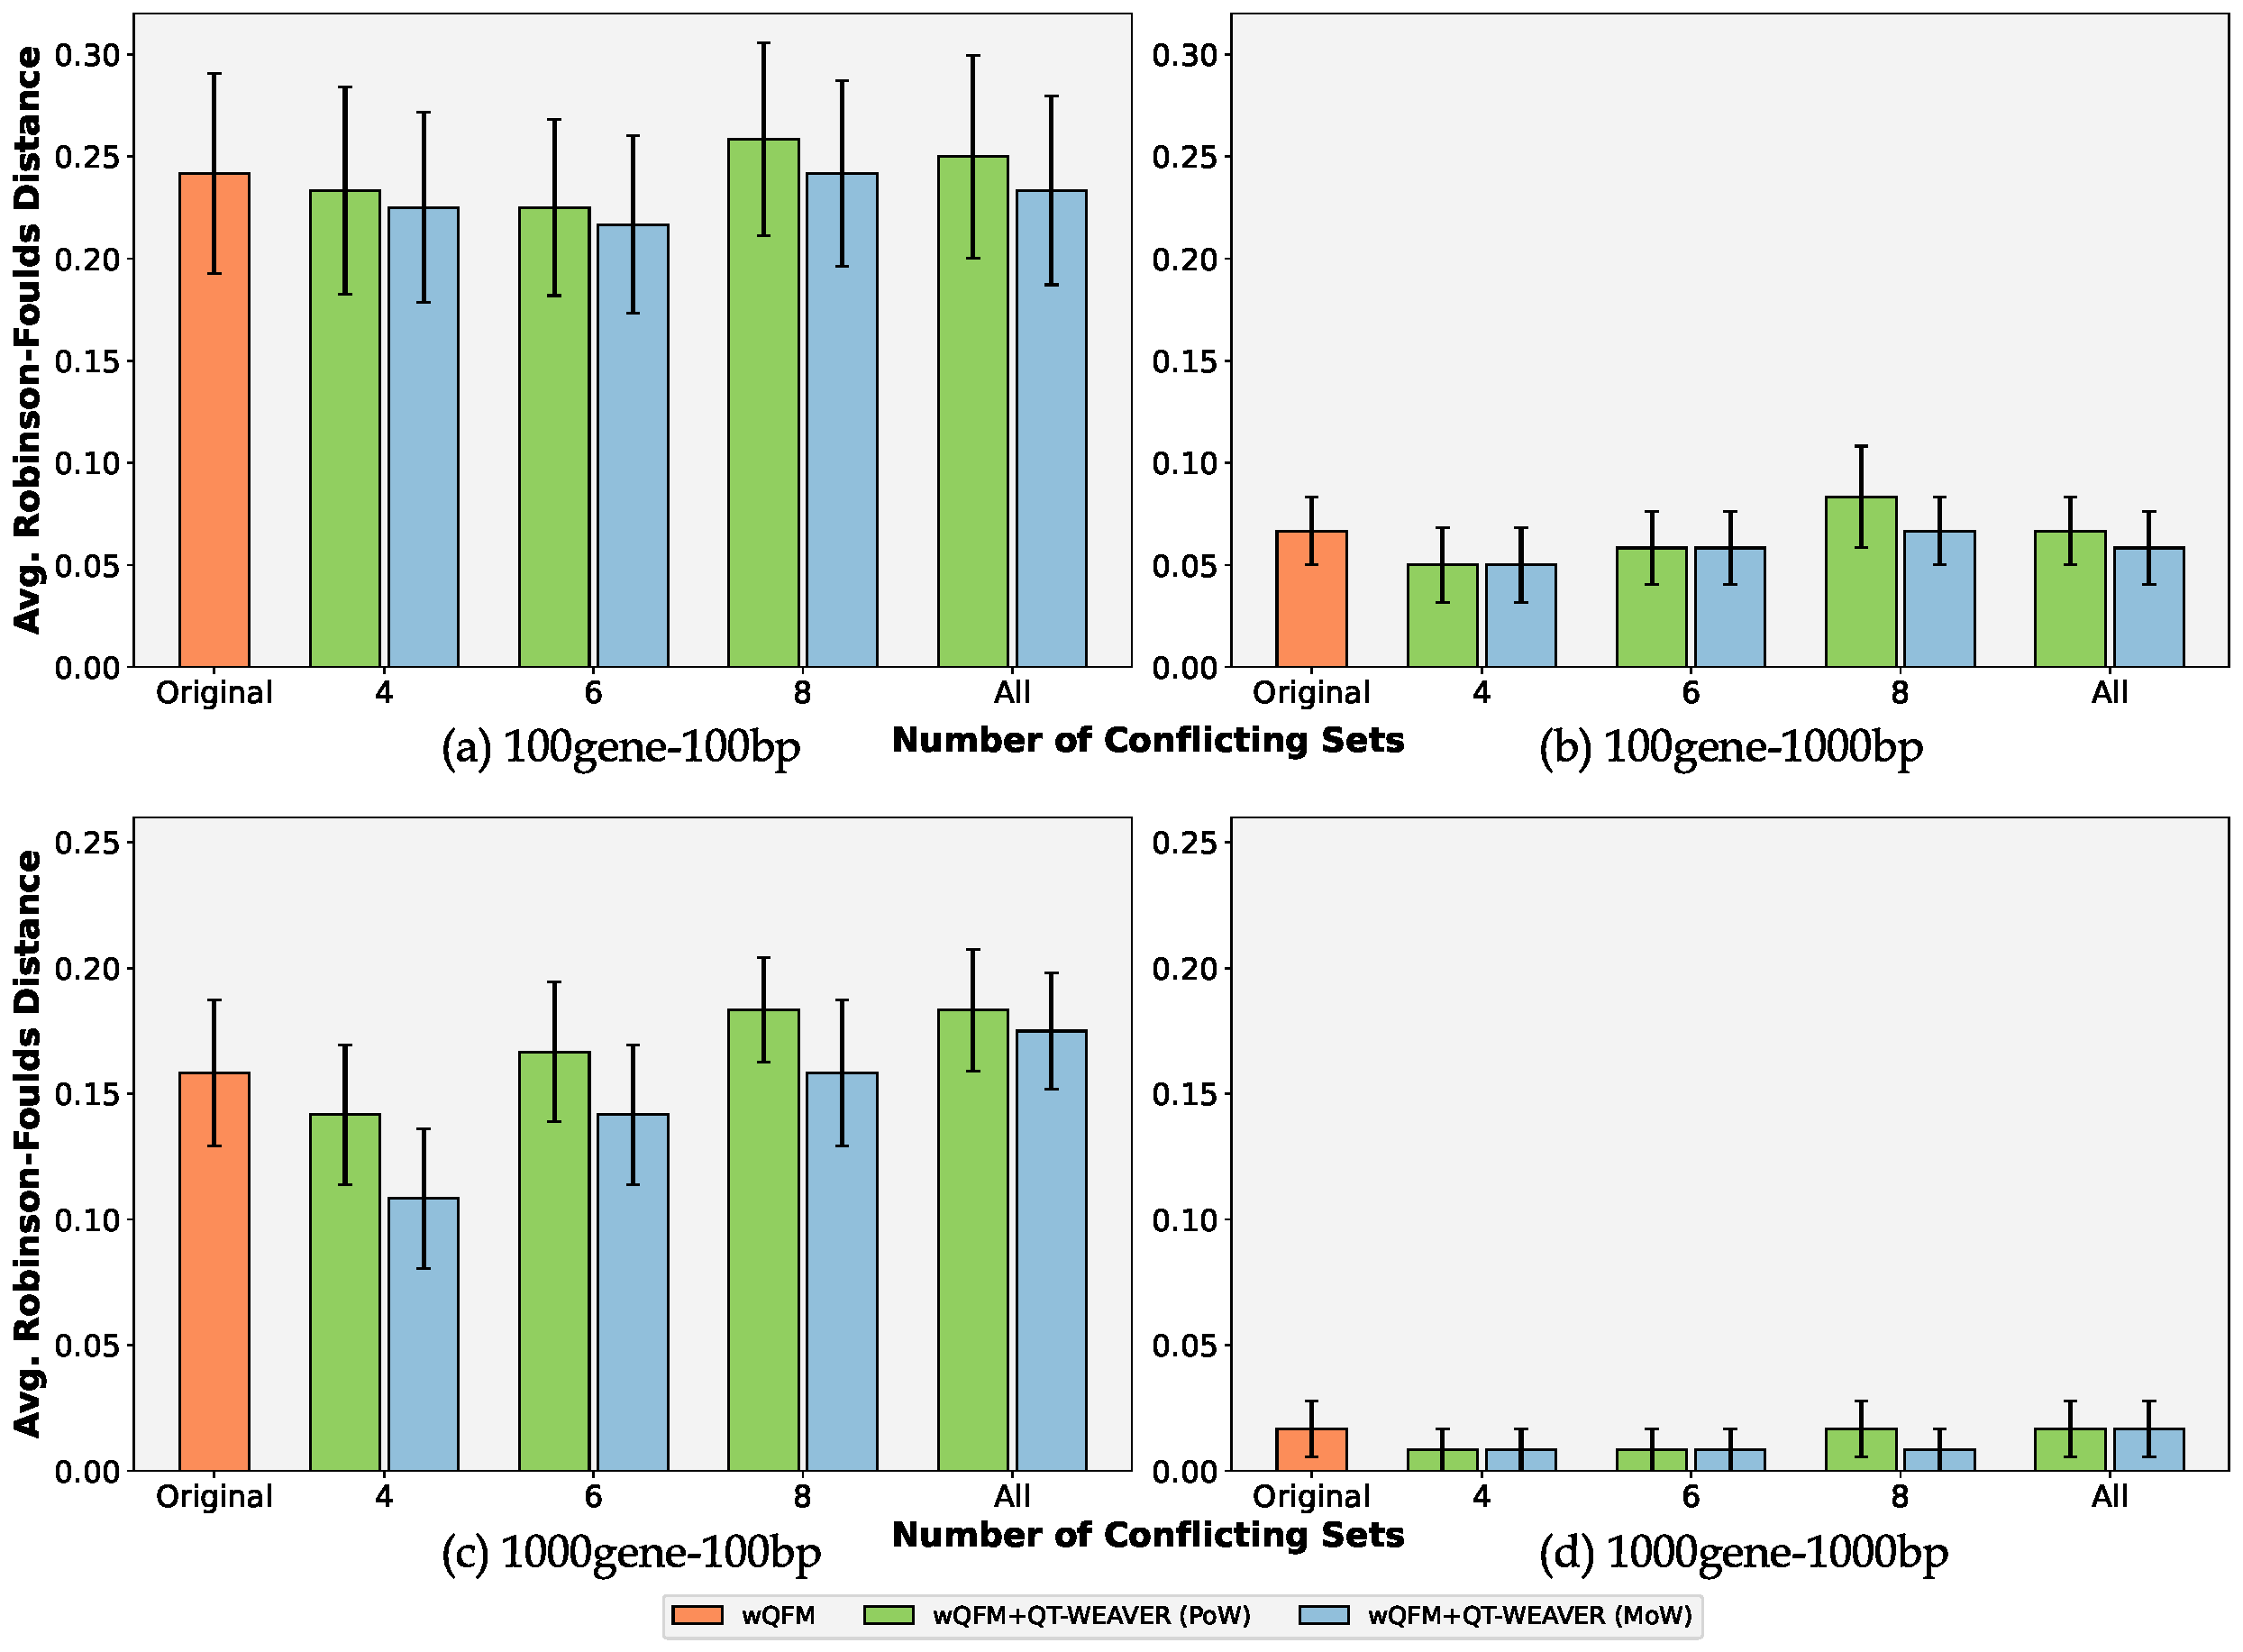
\includegraphics[width=.95\linewidth]{figures_new/1_15_modes.pdf}
    \caption{\textbf{Results on 15-taxon dataset.} Comparison of performance after correcting the weighted distributions using four, six, eight, and all 28 conflicting sets. We report the RF rates averaged over 10 replicates with standard errors. The distributions were amalgamated using wQFM. We show the effects of using both PoW and MoW weighting schemes. }
    \label{fig:rf_15_taxon_schemes}
\end{figure}

These results raise the question -- why does considering a small subset of all conflicting sets tend to yield better results? We hypothesize that using all 28 conflicting sets may impose excessive topological constraints on a quartet, making it challenging for QT-WEAVER to effectively distinguish among different topological variants.

In contrast, the six selected conflicting sets (as listed in Table \ref{table:conflicttable_six}) appear suitable for assessing conflict levels across quartet topologies, as indicated by our experimental results. While this specific choice of six sets lacks theoretical backing, we anticipate that the optimal subset--both in size and composition--may vary by dataset. Thus, an important research avenue involves automating the selection of these subsets, tailored to the topological features of the input gene trees, to optimize performance.

\begin{table}[h!]
\caption{We list the six conflicting sets chosen from all the conflicting sets in Table \ref{journal-table:conflicttable} from the main paper.}
    \centering
     \renewcommand{\arraystretch}{1.2}
    \begin{tabular}{|c|c|}
        \hline
        \textbf{Canonical Pair} & \textbf{Conflicting Quartets} \\ \hline

        $ab|cd$ \& $ac|be$ 
        & $ab|de$ $||$ $ae|bd$\\ \hline

        $ab|cd$ \& $ae|bc$ 
        & $ad|be$\\ \hline

        $ab|cd$ \& $ac|de$ 
        & $bd|ce$ $||$ $be|cd$\\ \hline

        $ab|cd$ \& $ad|ce$ 
        & $bc|de$\\ \hline
        
    \end{tabular}
    \label{table:conflicttable_six}
\end{table}

%So, why is it that only considering a small subset of all conflicting sets tends to yield better results? We hypothesize that all 28 conflicting sets together might be enforcing too much topological constraint on a quartet. As a result, it becomes difficult for QT-WEAVER to differentiate very well between different topological variants.


%On the other hand, the six conflicting sets that we chose (as outlined in Table \ref{table:conflicttable_six}) seem to be appropriate for identifying the degree of conflicts for different quartet topologies (as demonstrated in our experiments). The choice of these exact six sets does not hold much theoretical ground (future studies need to investigate this), and -- we believe -- depending on the dataset, the optimal choice (both size and elements) may vary. Therefore, automatic selection of the size and elements of these subsets, based on the topological structures of the input gene trees, to optimize the results is an important research direction.


%The ``minimum" weighting scheme outperforms the "regular" weighting scheme on all occasions. Furthermore, considering four or six conflicting sets produces the best results; the set of all 28 conflicting sets yields decent species trees, too. 
%In the most difficult model condition (100gene-100bp), taking six conflicting sets turns out to be the best choice.

%As utilizing six conflicting sets is not only faster than considering all but also yields better performance across all model conditions, we will only use this method in subsequent analyses. Moreover, we will only use the ``minimum" weighting scheme due to its superiority over the ``regular" weighting scheme. From now on, ``wQFM + QT-WEAVER" will denote estimating trees using wQFM on distributions corrected by QT-WEAVER with the minimum weighting scheme using six conflicting sets.


\clearpage
% \newpage
\section{Dataset}
\label{app:dataset}

\begin{table}[htbp]
\caption{Properties of the simulated datasets. The level of ILS is presented in terms of the average topological distance between true gene trees and true species trees.}
\label{table.data-description}
\centering
\begin{tabular}{c c c c c c} 
 \hline
 Dataset & ILS level & \# genes & \# sites & \# Replicates & Ref.\\  [0.5ex]
 \hline\hline
% 10-taxon & 40\%, 84\% & 200 & 100 & 20 & \cite{bayzid2015weighted} \\
% \hline
% 11-taxon & 38\%, 85\% & 5 - 100 & 2000 & 20 & \cite{chung2011} \\
 %\hline
 15-taxon & 82\% & 100 - 1000 & 100 - 1000 & 10 & \cite{bayzid2015weighted}\\
 \hline
 37-taxon & 18\%, 32\%, 54\% & 100 - 500 & 50 -1000 & 20 & \cite{statistical-binning}\\
 \hline
 48-taxon & 35\%, 47\%, 59\% & 100 - 500 & 50 -1000 & 20 & \cite{statistical-binning}\\
 \hline
 
\end{tabular}
\end{table}

% \clearpage
\section{Additional Results}
\label{app:additional-results}

\subsection{Additional results on 37-taxon dataset}
\label{app:37-taxon}

\begin{table}[h!]
    \centering
    % \small
    % \tiny
    \caption{The Jensen-Shannon divergence with respect to the true gene trees for different model conditions averaged over all replicates. The best-performing method (i.e., the least amount of divergence) for each model condition has been highlighted in bold.}
    % \bigskip
    \label{tab:37-divergence}
    \begin{tabular}{|C{3cm}|C{3cm}|C{3cm}|}
        \hline
        \textbf{Model Condition} & \textbf{GTF} & \textbf{QT-WEAVER} \\
        \hline
        0.5X-200-500 & \textbf{0.038} & 0.044 \\
        \hline
        1X-100-500 & 0.072 & \textbf{0.067} \\
        \hline
        1X-200-25 & 0.354 & \textbf{0.345} \\
        \hline
        1X-200-50 & 0.3 & \textbf{0.287} \\
        \hline
        1X-200-250 & 0.118 & \textbf{0.097} \\
        \hline
        1X-200-500 & 0.063 & \textbf{0.058} \\
        \hline
        1X-200-1000 & \textbf{0.034} & 0.053 \\
        \hline
        1X-500-500 & 0.057 & \textbf{0.052} \\
        \hline
        2X-200-500 & 0.097 & \textbf{0.082} \\
        \hline
    \end{tabular}
\end{table}

\begin{table}[h!]
    \centering
    % \small
    % \tiny
    \caption{Average quartet scores of estimated species trees and the true tree with respect to the estimated gene trees for the 37-taxon dataset. For wQFM+QT-WEAVER, we also report the quartet score with respect to the corrected estimated quartet distribution. The highest scores among the estimated trees have been italicized, and the scores closest to the true tree are shown in bold.}
    % \bigskip
    \label{tab:37-quartet-scores-estimated}
    \begin{tabular}{|C{2cm}|C{2.5cm}|C{2.5cm}|C{2.5cm}|C{2.5cm}|C{2.5cm}|}
        \hline
        \textbf{Model Condition} & \textbf{ASTRAL} & \textbf{wQFM} & \textbf{wQFM+QT-WEAVER (Original Distribution)} & \textbf{wQFM+QT-WEAVER (Corrected Distribution)} & \textbf{True Tree} \\
        \hline \hline
        0.5X-200-500 & 10007426 & 10006594 & \textbf{10006474} & \textit{10415670} & 10003930 \\
        \hline
        1X-100-500 & 5640132 & 5639605 & \textbf{5639168} & \textit{5806039} & 5636884 \\
        \hline
        1X-200-25 & 6491920 & 6489889 & \textbf{6489155} & \textit{6662792} & 6481431 \\
        \hline
        1X-200-50 & 7525465 & \textbf{7523379} & 7523903 & \textit{7778394} & 7517956 \\
        \hline
        1X-200-250 & 10569844 & 10568958 & \textbf{10568350} & \textit{10941339} & 10565292 \\
        \hline
        1X-200-500 & 11271938 & 11271426 & \textbf{11270680} & \textit{11603816} & 11267991 \\
        \hline
        1X-200-1000 & 11586641 & 11586355 & \textbf{11585945} & \textit{11886743} & 11584970 \\
        \hline
        1X-500-500 & 28171698 & \textbf{28171682} & 28168879 & \textit{28983587} & 28171386 \\
        \hline
        2X-200-500 & 11947266 & \textbf{11947020} & 11945419 & \textit{12175146} & 11946371 \\
        \hline
    \end{tabular}
\end{table}


\begin{table}[h!]
    \centering
    % \small
    % \tiny
    \caption{Average quartet scores of estimated species trees and the true tree with respect to the true gene trees for the 37-taxon dataset. The highest scores among the estimated trees have been italicized, and the scores closest to the true tree are shown in bold. %\add{Unlike Table \ref{tab:37-quartet-scores-estimated}, we could not report scores with respect to the corrected distribution, as we did not correct the true distribution (it has no GTEE).} \addb{But, didn't we show it in Figure \ref{fig:rf_37_taxon_methods}(c)?}
    }
    % \bigskip
    \label{tab:37-quartet-scores-true}
    \begin{tabular}{|C{2.3cm}|C{3cm}|C{3cm}|C{3cm}|C{3cm}|}
        \hline
        \textbf{Model Condition} & \textbf{ASTRAL} & \textbf{wQFM} & \textbf{wQFM+QT-WEAVER} & \textbf{True Tree} \\
        \hline \hline
        0.5X-200-500 & \textbf{\textit{10311630}} & 10311452 & 10311480 & 10311622 \\
        \hline
        1X-100-500 & 5870845 & 5871208 & \textbf{\textit{5871324}} & 5874698 \\
        \hline
        1X-200-25 & \textbf{\textit{11637683}} & 11613065 & 11627649 & 11744079 \\
        \hline
        1X-200-50 & 11688779 & \textbf{\textit{11707476}} & 11703316 & 11744079 \\
        \hline
        1X-200-250 & 11733853 & \textbf{\textit{11735693}} & 11731082 & 11744079 \\
        \hline
        1X-200-500 & 11738631 & 11739572 & \textbf{\textit{11741356}} & 11744079 \\
        \hline
        1X-200-1000 & 11743809 & 11743721 & \textbf{\textit{11744134}} & 11744079 \\
        \hline
        1X-500-500 & 29362939 & \textbf{\textit{29363114}} & 29356078 & 29364014 \\
        \hline
        2X-200-500 & 12565282 & \textbf{\textit{12565347}} & 12563879 & 12570343 \\
        \hline
    \end{tabular}
\end{table}


\begin{figure}[h]
    \centering % <-- added
    % 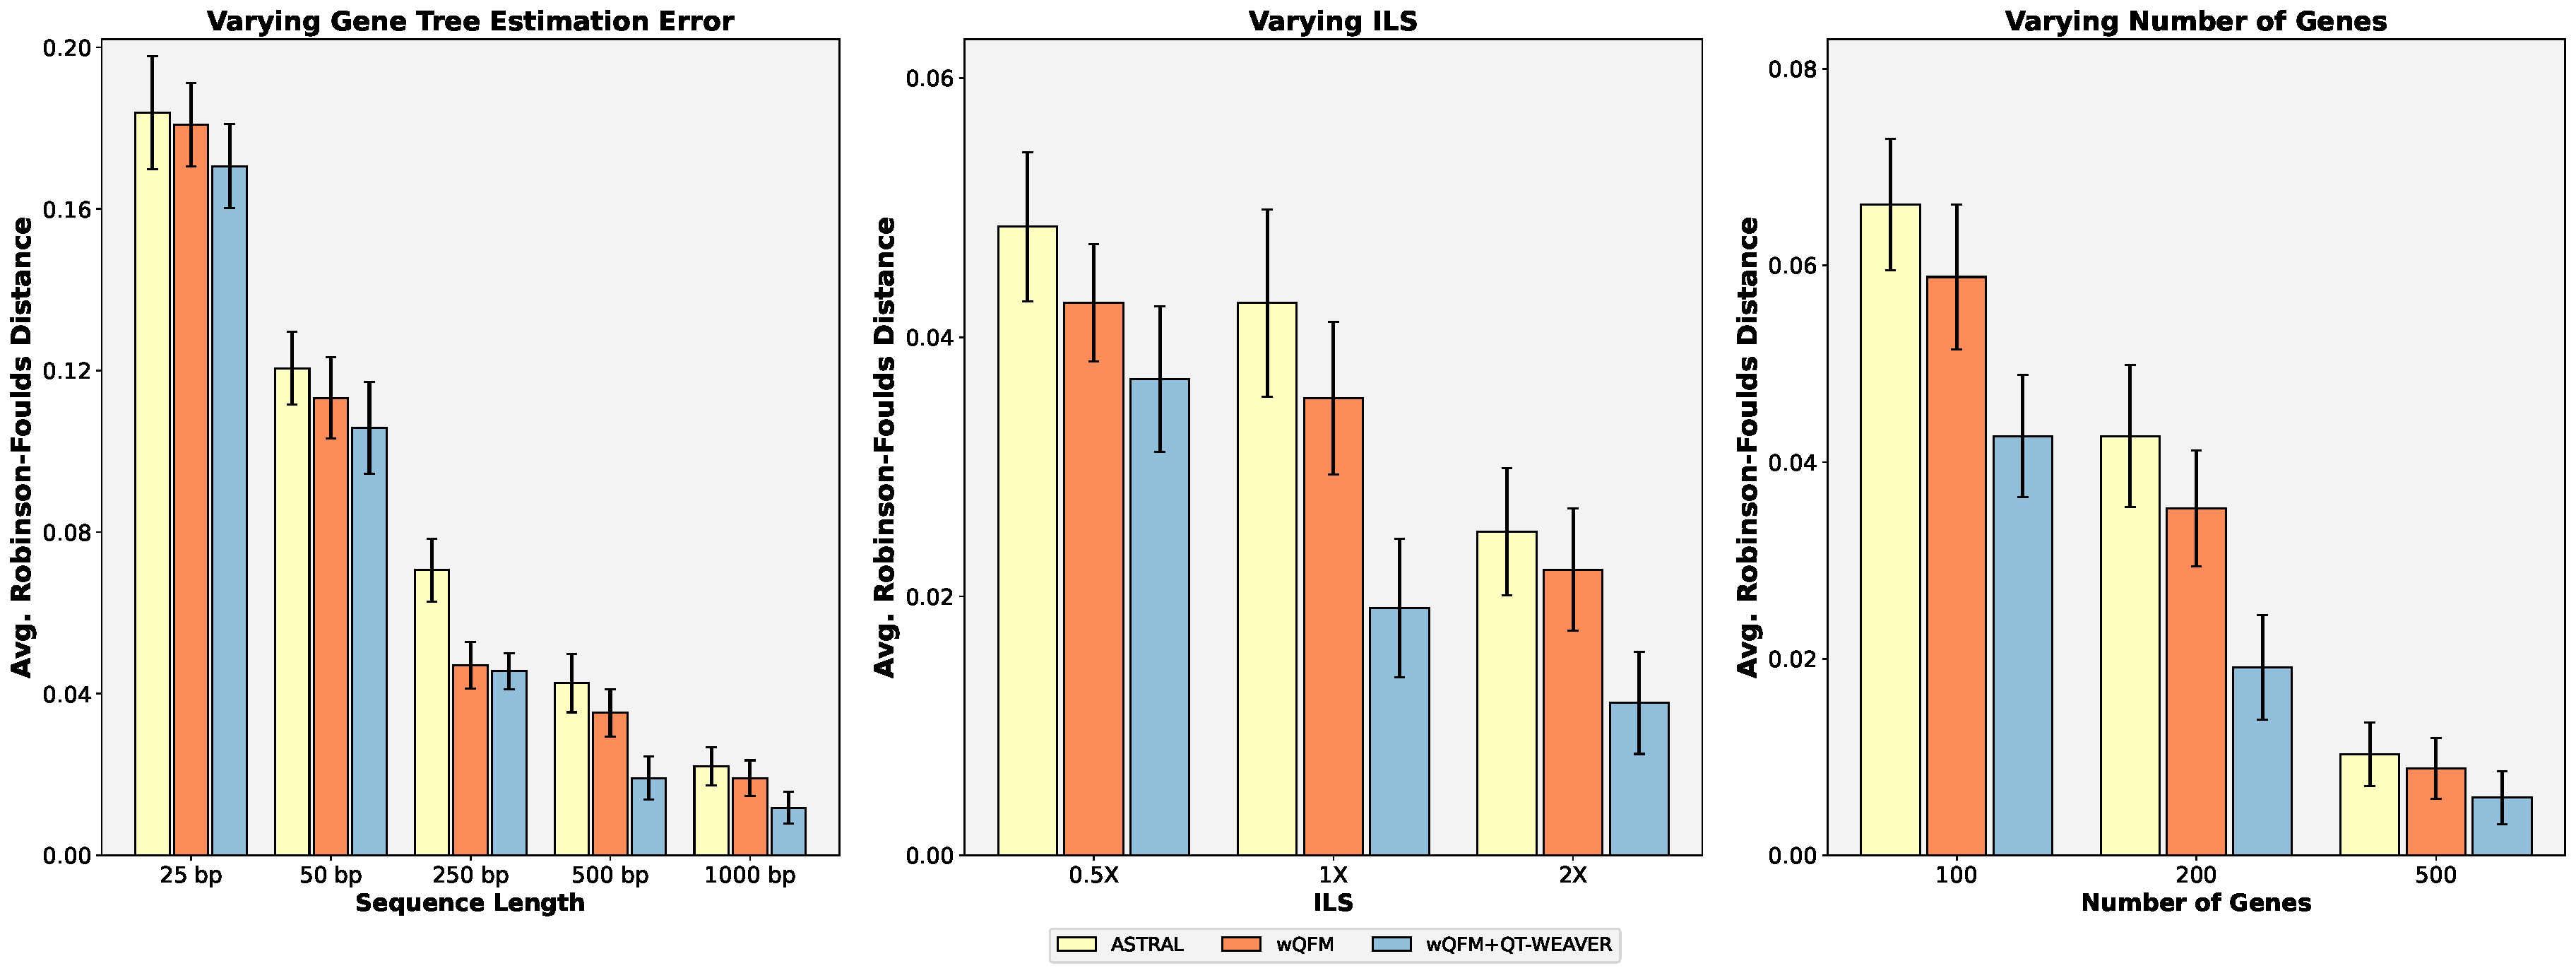
\includegraphics[width=\linewidth]{figures_new/2_37_methods.pdf}
    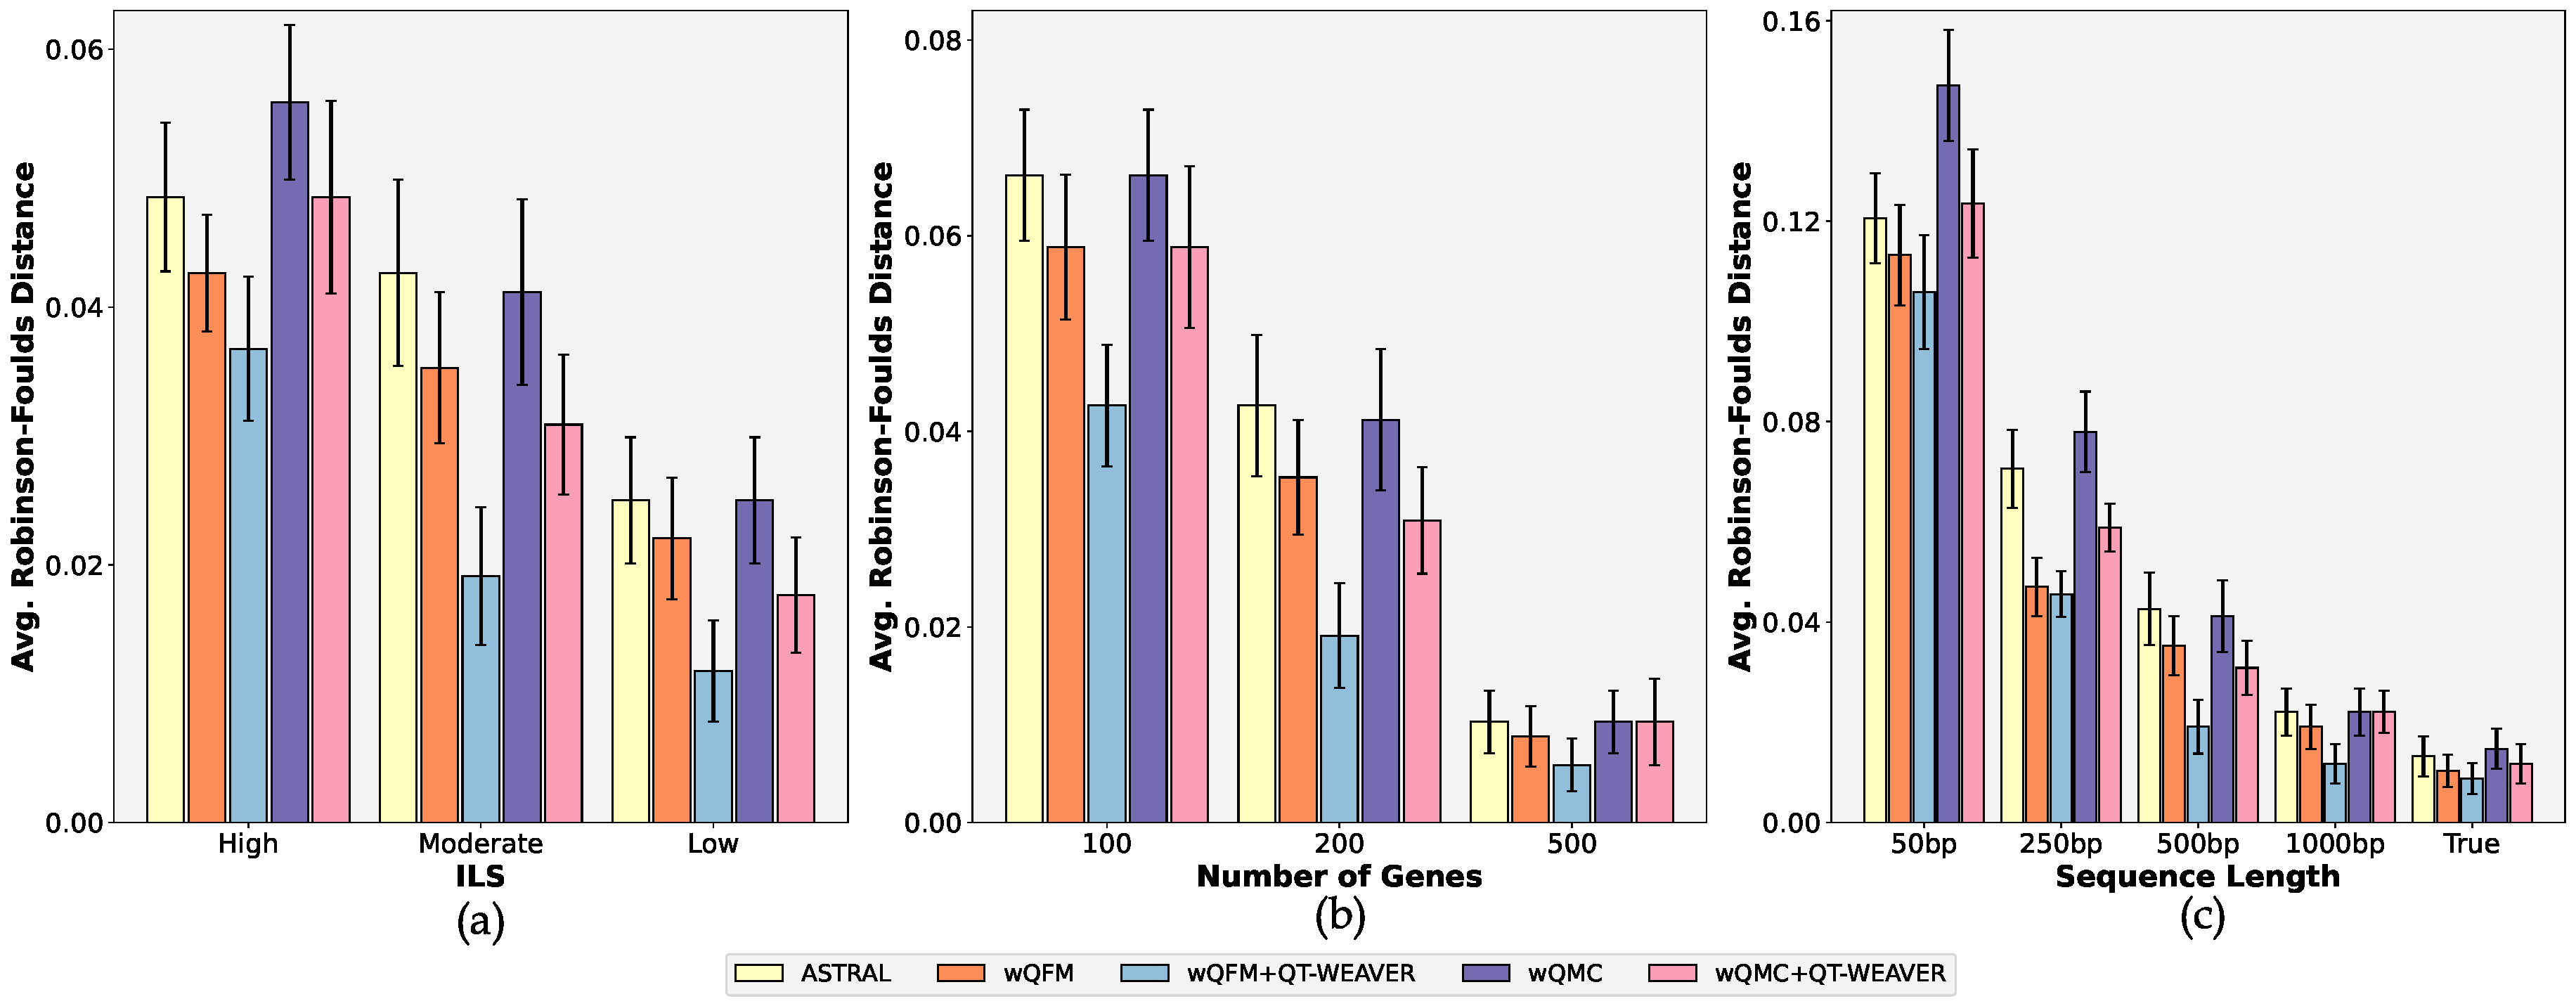
\includegraphics[width=\linewidth]{figures_new/9_37_methods_wqmc.pdf}
    \caption{\textbf{Results on 37-taxon dataset.} We show the average RF rates with standard errors over 20 replicates for the methods ASTRAL, wQFM (wQFM-uncorrected), wQFM+QT-WEAVER (wQFM-corrected), wQMC (wQMC-uncorrected), and wQMC+QT-WEAVER (wQMC-corrected). The settings in (a)-(c) are identical to the ones in Figure \ref{journal-fig:rf_37_taxon_methods} in the main paper. }
    \label{fig:rf_37_taxon_wqmc}
\end{figure}

\newpage

\subsection{Additional results on 15-taxon dataset}
\label{app:15-taxon}

% \begin{figure}[h!]
%     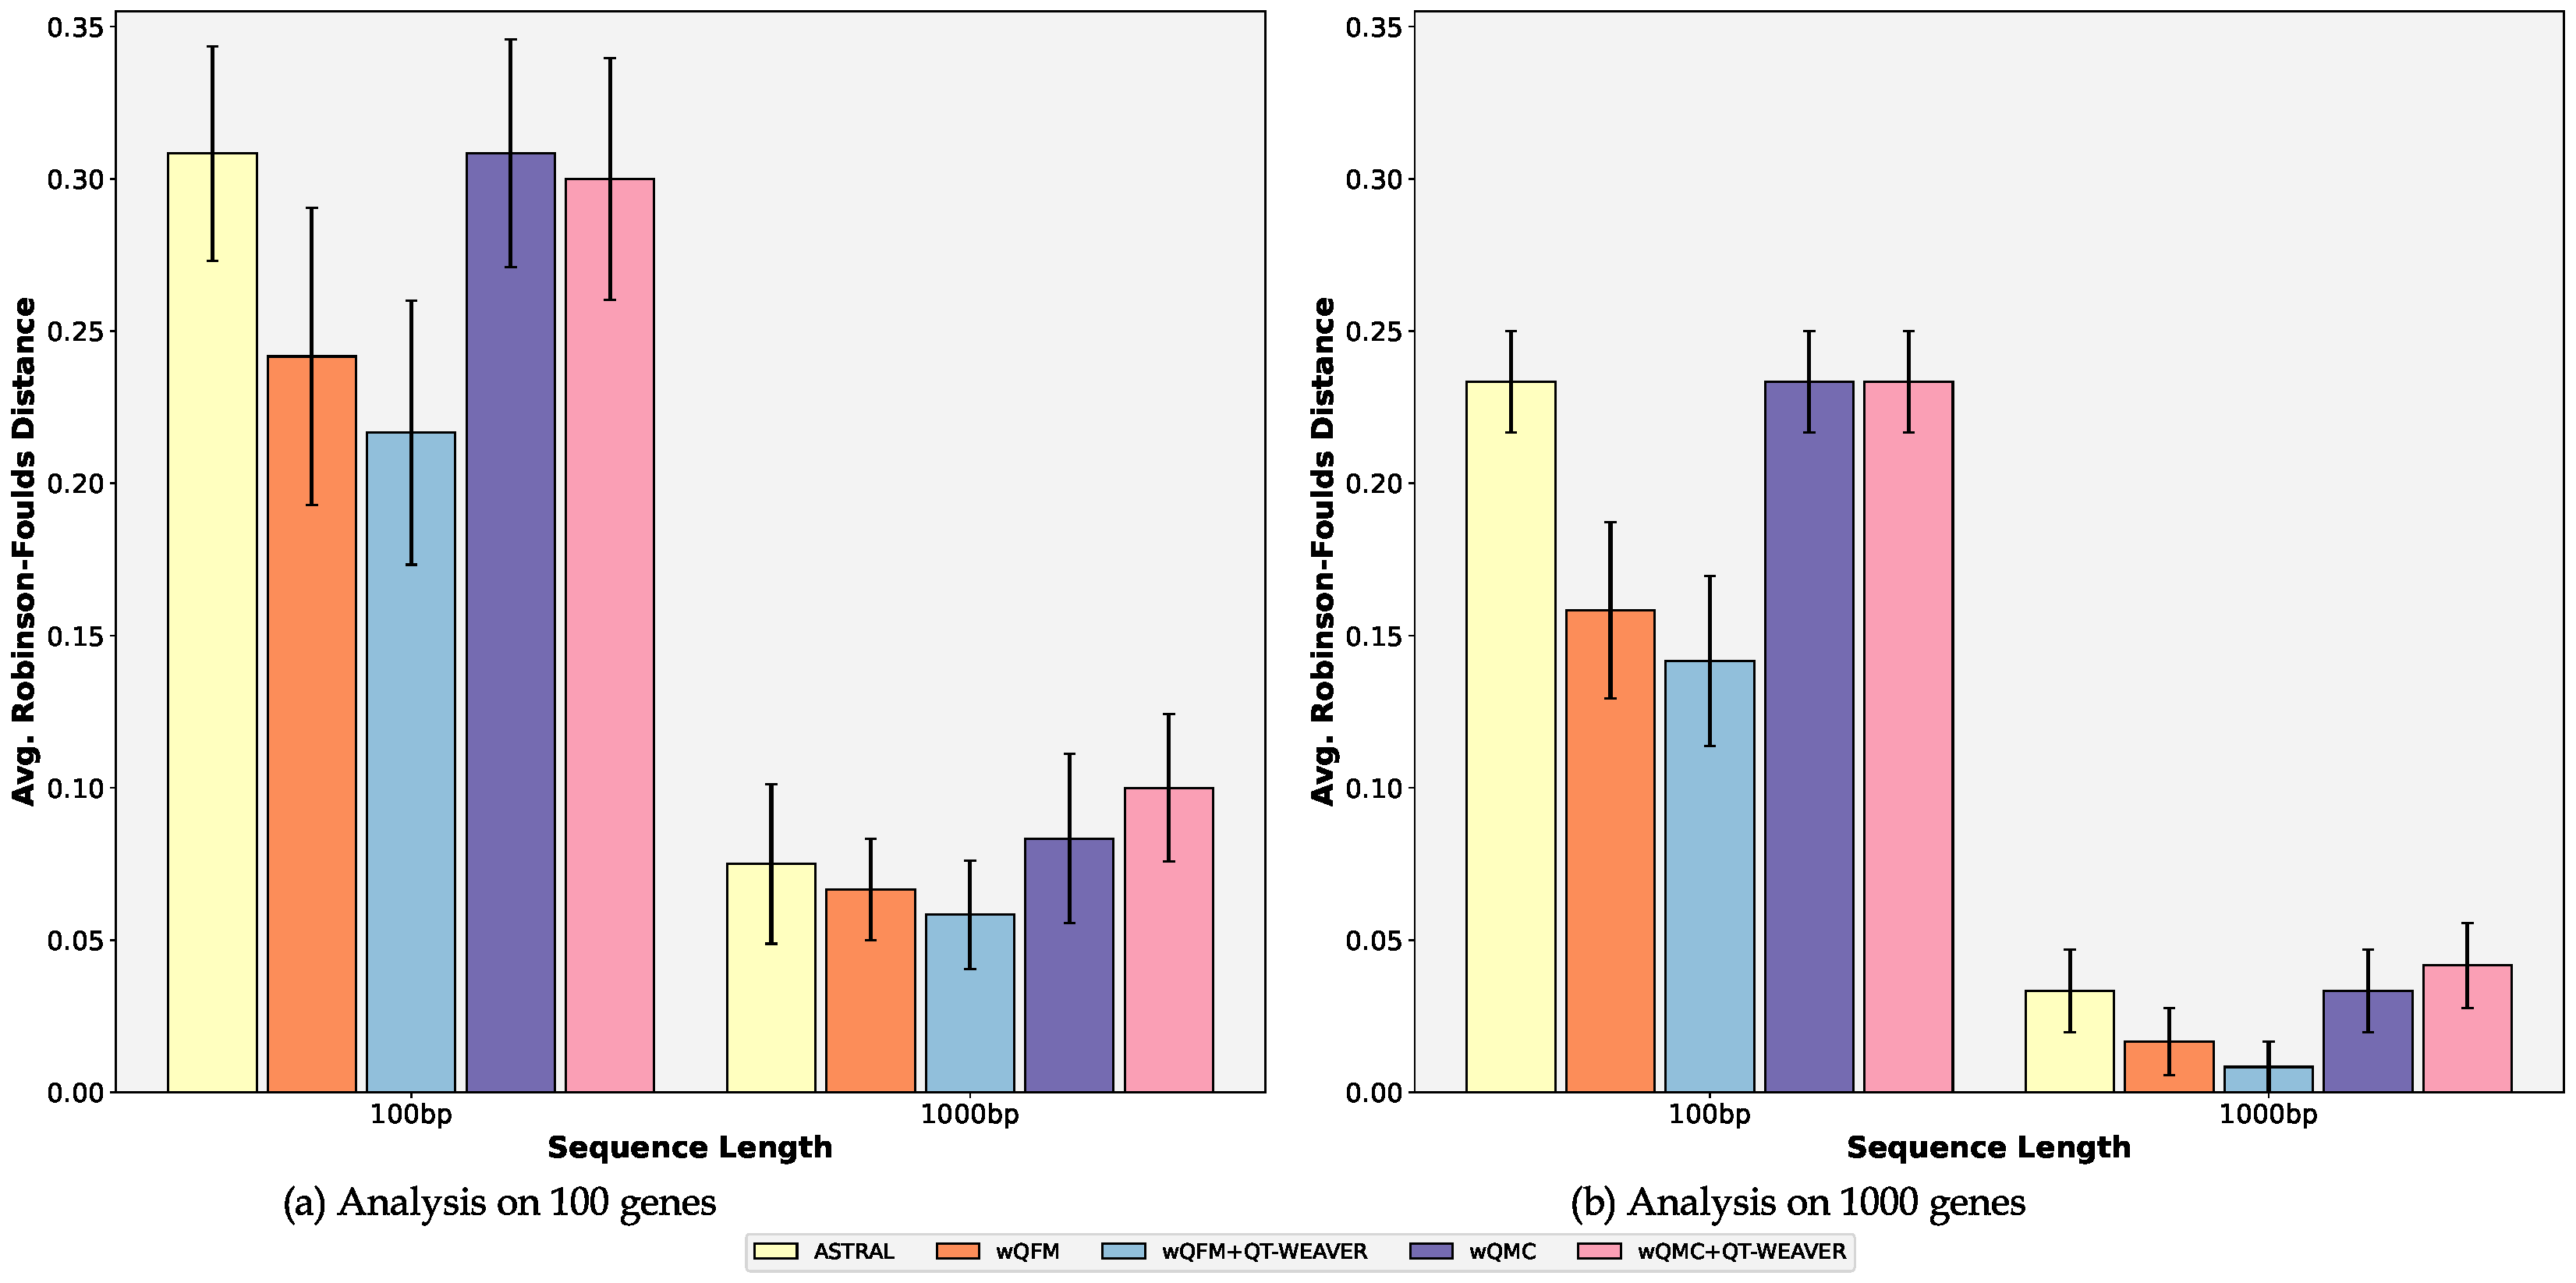
\includegraphics[width=\linewidth, height=0.5\linewidth]{figures_new/9_15_methods_wqmc.pdf}
%     \caption{\textbf{Results on 15-taxon dataset.} (a)-(b) We compare the average RF distance of ASTRAL, wQFM, wQFM+QT-WEAVER, wQMC, and wQMC+QT-WEAVER on varying model conditions. The settings are identical to the ones in Figure \ref{fig:rf_15_taxon_methods}.}
%     \label{fig:rf_15_taxon_methods_wqmc}
% \end{figure}


\begin{table}[h!]
    \centering
    % \small
    % \tiny
    \caption{The Jensen-Shannon divergence with respect to the true gene trees for different model conditions averaged over all replicates. The best-performing method (i.e., the least amount of divergence) for each model condition has been highlighted in bold.}
    % \bigskip
    \label{tab:15-divergence}

    \begin{tabular}{|c|C{3cm}|C{3cm}|}
        \hline
        \textbf{Model Condition} & \textbf{GTF} & \textbf{QT-WEAVER} \\
        \hline
        100gene-100bp & 0.115 & \textbf{0.103} \\
        \hline
        100gene-1000bp & \textbf{0.043} & 0.049 \\
        \hline
        1000gene-100bp & 0.101 & \textbf{0.087} \\
        \hline
        1000gene-1000bp & \textbf{0.031} & 0.037 \\
        \hline
    \end{tabular}
\end{table}

\begin{table}[h!]
    \centering
    % \small
    % \tiny
    \caption{Average quartet scores of estimated species trees and the true tree with respect to the estimated gene trees for the 15-taxon dataset. For wQFM+QT-WEAVER, we also report the quartet score with respect to the corrected estimated quartet distribution. The highest scores among the estimated trees have been italicized, and the scores closest to the true tree are shown in bold.}
    % \bigskip
    \label{tab:15-quartet-scores-estimated}
    \begin{tabular}{|C{2cm}|C{2.5cm}|C{2.5cm}|C{2.5cm}|C{2.5cm}|C{2.5cm}|}
        \hline
        \textbf{Model Condition} & \textbf{ASTRAL} & \textbf{wQFM} & \textbf{wQFM+QT-WEAVER (Original Distribution)} & \textbf{wQFM+QT-WEAVER (Corrected Distribution)} & \textbf{True Tree} \\
        \hline \hline
        100gene-100bp & 69934 & \textbf{69777} & 69792 & \textit{73598} & 69307 \\
        \hline
        100gene-1000bp & 82167 & 82129 & \textbf{82125} & \textit{87562} & 82099 \\
        \hline
        1000gene-100bp & 693656 & 692949 & \textbf{692664} & \textit{727712} & 690268 \\
        \hline
        1000gene-1000bp & 818022 & 817994 & \textbf{817953} & \textit{869904} & 817937 \\
        \hline
    \end{tabular}
\end{table}

\begin{table}[h!]
    \centering
    % \small
    % \tiny
    \caption{Average quartet scores of estimated species trees and the true tree with respect to the true gene trees for the 15-taxon dataset. The highest scores among the estimated trees have been italicized, and the scores closest to the true tree are shown in bold.}
    % \bigskip
    \label{tab:15-quartet-scores-true}
    \begin{tabular}{|C{2.3cm}|C{3cm}|C{3cm}|C{3cm}|C{3cm}|}
        \hline
        \textbf{Model Condition} & \textbf{ASTRAL} & \textbf{wQFM} & \textbf{wQFM+QT-WEAVER} & \textbf{True  Tree} \\
        \hline \hline
        100gene-100bp & 82159 & 82708 & \textbf{\textit{83078}} & 84635 \\
        \hline
        100gene-1000bp & 84345 & 84437 & \textbf{\textit{84444}} & 84635 \\
        \hline
        1000gene-100bp & 827970 & 834890 & \textbf{\textit{836349}} & 844184 \\
        \hline
        1000gene-1000bp & 843363 & 843792 & \textbf{\textit{843973}} & 844184 \\
        \hline
    \end{tabular}
\end{table}

%On the other hand, maximizing the quartet scores with respect to the estimated gene trees may not guarantee more accuracy in the presence of gene tree estimation errors and limited number of genes. The true tree having the lowest quartet scores across all model conditions supports this claim (Table \ref{tab:15-quartet-scores-estimated}). ASTRAL attains the highest quartet scores, which is furthest from the true tree, suggesting that it is ``overshooting" the quartet scores as it returns the least accurate tree among the three methods. Clearly, the wQFM+QT-WEAVER species trees, when compared to the original estimated distribution, are suffering from this ``overshooting" issue the least, which results in the best trees. Interestingly, when we consider the ``corrected" estimated distribution, the quartet scores of wQFM+QT-WEAVER are by far the highest, indicating that the corrected distribution was able to shed much of the limitations caused by gene tree estimation error and a limited number of genes. Hence, the corrected distribution is a more reliable representation of the true distribution.

\clearpage

\subsection{Additional results on 48-taxon dataset}
\label{app:48-taxon}
\begin{table}[h!]
    \centering
    % \small
    % \tiny
    \caption{The Jensen-Shannon divergence with respect to the true gene trees for different model conditions averaged over all replicates. The best-performing method (i.e., the least amount of divergence) for each model condition has been highlighted in bold.}
    % \bigskip
    \label{tab:48-divergence}

    \begin{tabular}{|c|C{3cm}|C{3cm}|}
        \hline
        \textbf{Model Condition} & \textbf{GTF} & \textbf{QT-WEAVER} \\
        \hline
        0.5X-1000-500 & 0.053 & \textbf{0.05} \\
        \hline
        1X-50-500 & 0.119 & \textbf{0.115} \\
        \hline
        1X-100-500 & 0.104 & \textbf{0.1} \\
        \hline
        1X-200-500 & 0.095 & \textbf{0.09} \\
        \hline
        1X-500-500 & 0.088 & \textbf{0.084} \\
        \hline
        1X-1000-500 & 0.086 & \textbf{0.082} \\
        \hline
        2X-1000-500 & 0.129 & \textbf{0.125} \\
        \hline
    \end{tabular}
\end{table}

\begin{table}[h!]
    \centering
    % \small
    % \tiny
    \caption{Average quartet scores of estimated species trees and the true tree with respect to the estimated gene trees for the 48-taxon dataset. For wQFM+QT-WEAVER, we also report the quartet score with respect to the corrected estimated quartet distribution. The highest scores among the estimated trees have been italicized, and the scores closest to the true tree are shown in bold.}
    % \bigskip
    \label{tab:48-quartet-scores-estimated}
    \begin{tabular}{|C{2cm}|C{2.5cm}|C{2.5cm}|C{2.5cm}|C{2.5cm}|C{2.5cm}|}
        \hline
        \textbf{Model Condition} & \textbf{ASTRAL} & \textbf{wQFM} & \textbf{wQFM+QT-WEAVER (Original Distribution)} & \textbf{wQFM+QT-WEAVER (Corrected Distribution)} & \textbf{True Tree} \\
        \hline \hline
        0.5X-1000-500 & 110583149 & 110590454 & \textbf{110571852} & \textit{111644682} & 110526513 \\
        \hline
        1X-50-500 & 6204884 & 6191081 & \textbf{6188251} & \textit{6301099} & 6109255 \\
        \hline
        1X-100-500 & 12349311 & \textbf{12324222} & 12328065 & \textit{12509069} & 12250259 \\
        \hline
        1X-200-500 & 24632824 & 24606334 & \textbf{24602225} & \textit{24885625} & 24553381 \\
        \hline
        1X-500-500 & \textbf{3106420} & 3101726 & 3107694 & \textit{3134254} & 3104926 \\
        \hline
        1X-1000-500 & 123024938 & 122994498 & \textbf{122983971} & \textit{124026278} & 122945091 \\
        \hline
        2X-1000-500 & 131631394 & 131619670 & \textbf{131603624} & \textit{132583373} & 131567523 \\
        \hline
    \end{tabular}
\end{table}

\begin{table}[h!]
    \centering
    % \small
    % \tiny
    \caption{Average quartet scores of estimated species trees and the true tree with respect to the true gene trees for the 48-taxon dataset. The highest scores among the estimated trees have been italicized, and the scores closest to the true tree are shown in bold.}
    % \bigskip
    \label{tab:48-quartet-scores-true}
    \begin{tabular}{|C{2.3cm}|C{3cm}|C{3cm}|C{3cm}|C{3cm}|}
        \hline
        \textbf{Model Condition} & \textbf{ASTRAL} & \textbf{wQFM} & \textbf{wQFM+QT-WEAVER} & \textbf{True  Tree} \\
        \hline \hline
        0.5X-1000-500 & 119513732 & 119525755 & \textbf{\textit{119540365}} & 119669367 \\
        \hline
        1X-50-500 & 6746768 & 6743642 & \textbf{\textit{6753059}} & 6789683 \\
        \hline
        1X-100-500 & 13506775 & 13506470 & \textbf{\textit{13513183}} & 13610325 \\
        \hline
        1X-200-500 & \textbf{\textit{27093454}} & 27091736 & 27086810 & 27229537 \\
        \hline
        1X-500-500 & \textbf{\textit{3418291}} & 3415138 & 3417996 & 3424968 \\
        \hline
        1X-1000-500 & 135991280 & \textbf{\textit{136016624}} & 136009169 & 136107790 \\
        \hline
        2X-1000-500 & \textbf{\textit{148393885}} & 148377461 & 148321043 & 148466576 \\
        \hline
    \end{tabular}
\end{table}

% \newpage
\clearpage

% \subsection{Additional results on iterative corrections using QT-WEAVER}
% \label{app:iterations}

% We investigated how the Jensen-Shannon divergence evolves across iterations (see Figure \ref{fig:rf_15_taxon_iterative_2}(a) in Appendix \ref{app:iterations}). Initially, the divergence decreases during the first one or two iterations but then begins to increase. This occurs because, for the three alternative quartet topologies ($ab|cd, ac|bd, ad|bc$) on four taxa, QT-WEAVER tends to prioritize the quartet topology it identifies as ``correct'' --the one with the least conflict score--by increasing its weight while reducing the weights of the alternative topologies.  Thus, with successive iterations, the weight of the ``correct'' quartet topology continues to rise (toward 100\%) while the weights of the other two alternatives keep decreasing (toward 0\%). Thus, this overestimation of the weight of the ``correct'' quartets and the underestimation of the weights of the ``incorrect'' ones lead the adjusted distribution to diverge from the true weighted distribution. Despite this divergence, the iterative adjustments may still guide the tree search algorithm toward more accurate trees (up to a certain point) by emphasizing and amalgamating the quartets with higher weights, as evidenced by the gradual decrease in the RF rates up to 10-15 iterations. For the same reason, when examining the quartet scores of wQFM+QT-WEAVER with respect to the corresponding corrected quartet distribution (instead of the original quartet distribution), the scores continue to increase, approaching nearly 100\% (see Figure \ref{fig:rf_15_taxon_iterative_2}(b) in Appendix \ref{app:iterations}). This occurs because, in the corrected distribution, the weights of the quartets present in the estimated species trees steadily rise, resulting in higher quartet scores for the estimated trees.


% \begin{figure}[h!]
%     \centering % <-- added
%     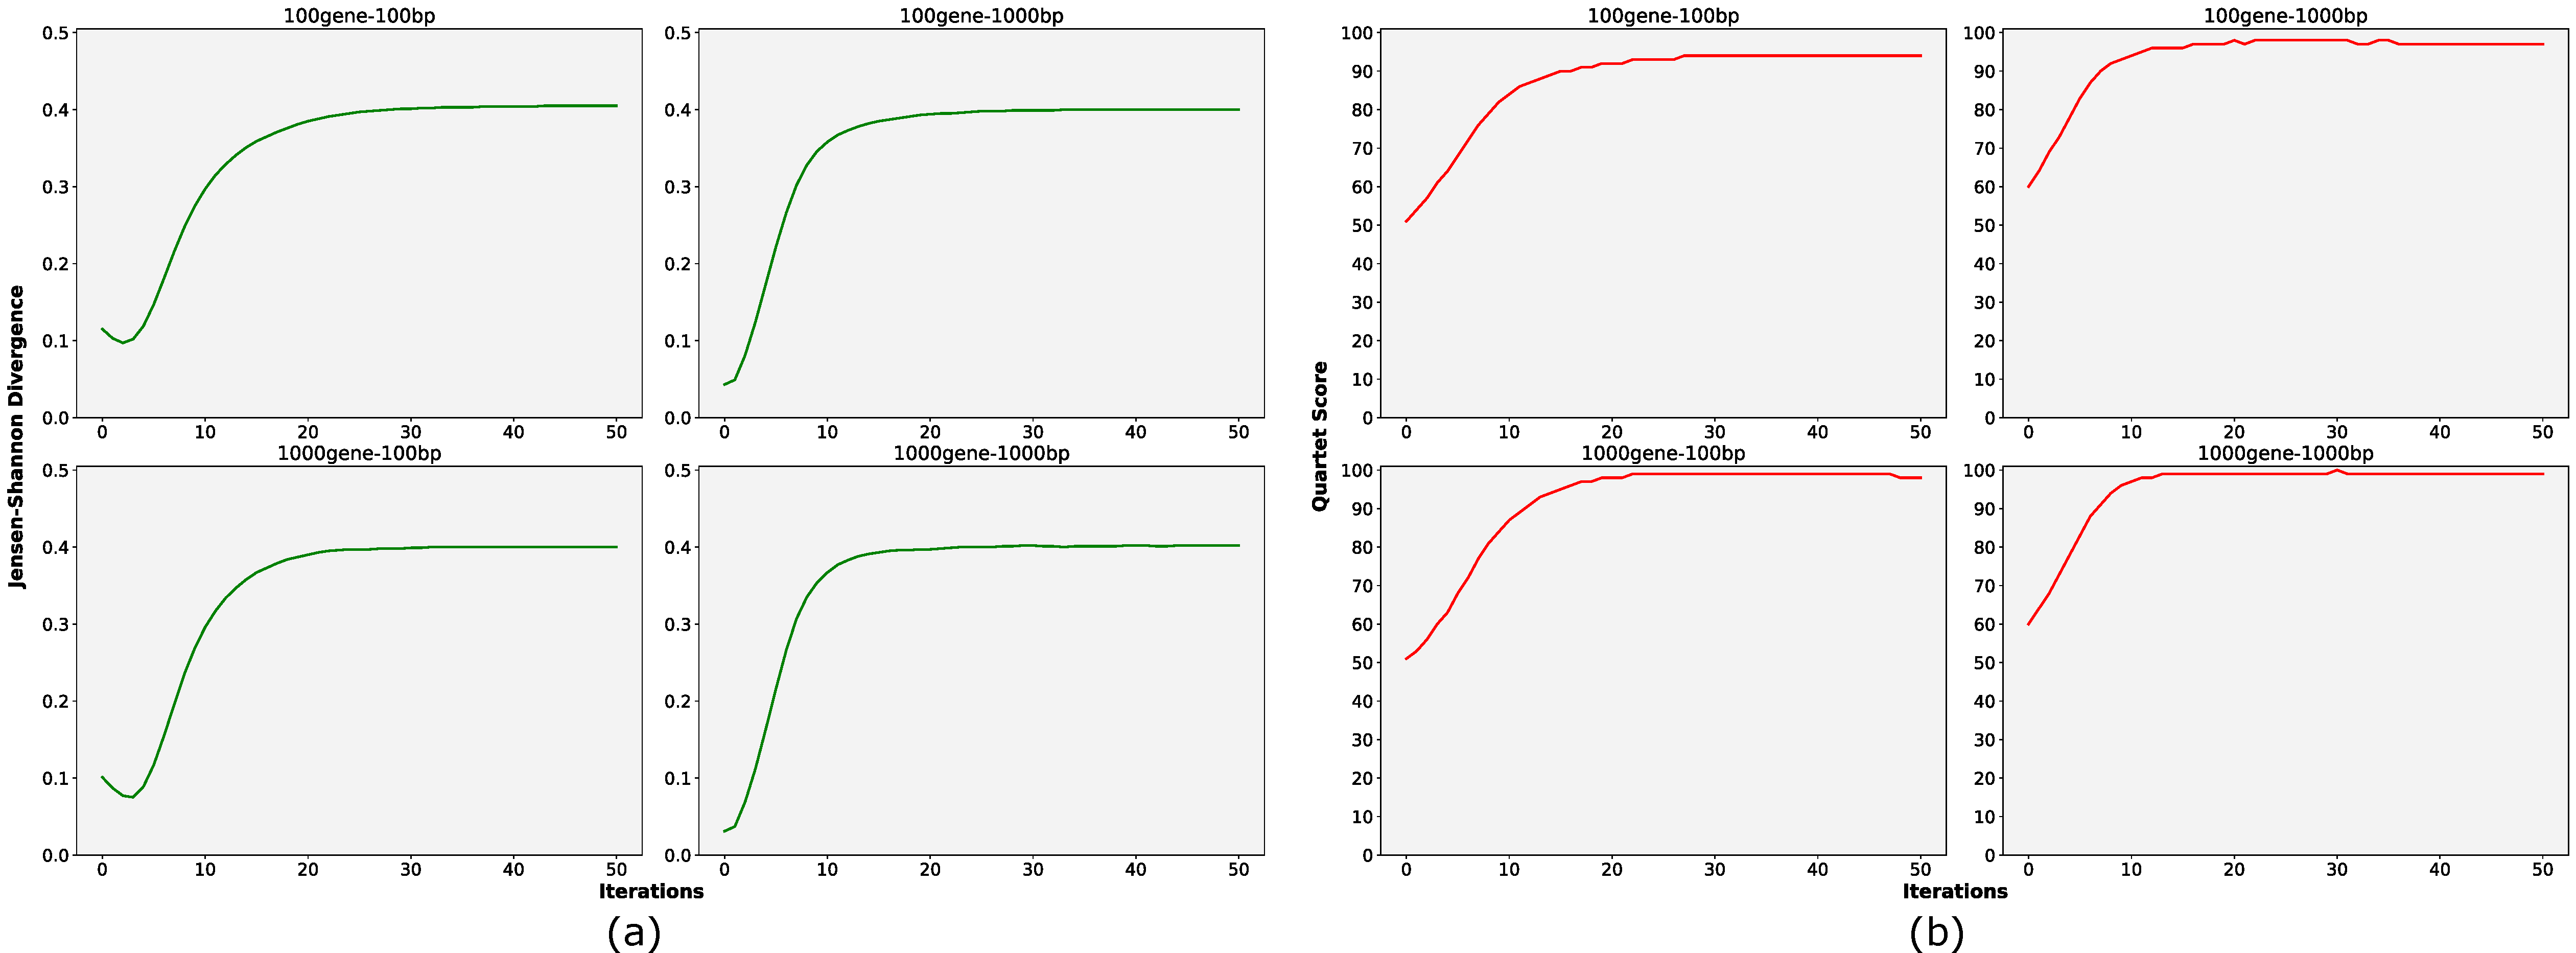
\includegraphics[width=\linewidth]{figures_new/15_iterative_2.pdf}
%     \caption{\textbf{Results iterative corrections on 15-taxon dataset.} We show the changes in (a) Jensen-Shannon divergence with respect to the true quartet distribution and (b) the quartet score of the estimated species tree with respect to its corresponding corrected quartet distribution over 50 iterations. 
%     }
%     \label{fig:rf_15_taxon_iterative_2}
% \end{figure}


% \subsection{Running time}
% \label{app:running-time}
% \begin{table}[htbp]
% \caption{Running time of QT-GILD for one epoch on different dataset.}
% \label{table.running time}
% \centering
% \begin{tabular}{c  c c } 
%  \toprule
%  Dataset &  \# Genes & Running time (seconds)  \\  [0.5ex]
%  \hline\hline
%  15-taxon & 100 & 25\times10^{-3} - 26\times10^{-3} \\
%  15-taxon & 1000 & 750\times10^{-3} - 800\times10^{-3} \\ \midrule
%  37-taxon & 100 & 1 $-$ 1.5\\
%  37-taxon & 200 & 2 $-$ 3\\
%  37-taxon & 400 & 5 $-$ 6\\ \midrule
%  Angiosperm (46-taxon) & 310 & 10 $-$ 11\\
%  \bottomrule
 
% \end{tabular}
% \end{table}

% \newpage

% \section{Analysis of Avian Biological Dataset}
% \label{app:avian-biological}


\bibliographystyle{unsrt}
% \bibliography{References}
\bibliographystyle{IEEEtran}
\bibliography{references.bib} % NEED TO CHANGE to references.bib

\end{document}
\newcommand{\quartet}[4]{
  \begin{tikzpicture}
    % Nodes
    \node (a) at (0, 2) {};
    \node (b) at (0, 0) {};
    \node (c) at (3, 2) {};
    \node (d) at (3, 0) {};
    \node (center1) at (1, 1) {};
    \node (center2) at (2, 1) {};
    \node (name) at (1.5, -0.5) {$#1#2|#3#4$};

    % Edges
    \draw[thick] (a) -- (center1);
    \draw[thick] (b) -- (center1);
    \draw[thick] (center1) -- (center2);
    \draw[thick] (center2) -- (c);
    \draw[thick] (center2) -- (d);

    % Dots at nodes
    \fill (a) circle (2pt);
    \fill (b) circle (2pt);
    \fill (c) circle (2pt);
    \fill (d) circle (2pt);
    \fill (center1) circle (2pt);
    \fill (center2) circle (2pt);

    % Labels
    \node at (-0.2, 2) {#1};
    \node at (3.2, 2) {#3};
    \node at (3.2, 0) {#4};
    \node at (-0.2, 0) {#2};
  \end{tikzpicture}
}

\newcommand{\fivetax}[5]{
\begin{tikzpicture}
% Nodes
\node (a) at (0, 2) {};
\node (b) at (0, 0) {};
\node (c) at (3, 2) {};
\node (d) at (3, 0) {};
\node (x) at (0.5, 1.5) {};
\node (e) at (0, 1) {};

\node (center1) at (1, 1) {};
\node (center2) at (2, 1) {};

% Edges
\draw[thick] (a) -- (x);
\draw[thick] (center1) -- (x);
\draw[thick] (b) -- (center1);
\draw[thick] (center1) -- (center2);
\draw[thick] (center2) -- (c);
\draw[thick] (center2) -- (d);
\draw[thick] (e) -- (x);

% Dots at nodes
\fill (a) circle (2pt);
\fill (b) circle (2pt);
\fill (c) circle (2pt);
\fill (d) circle (2pt);
\fill (x) circle (2pt);
\fill (e) circle (2pt);
\fill (center1) circle (2pt);
\fill (center2) circle (2pt);

% Labels
\node at (-0.2, 2) {#1};
\node at (3.2, 2) {#3};
\node at (3.2, 0) {#4};
\node at (-0.2, 0) {#2};
\node at (-0.2, 1) {#5};
\end{tikzpicture}
}

\newcommand{\fivetaxcol}[5]{
\begin{tikzpicture}
% Nodes
\node (a) at (0, 2) {};
\node (b) at (0, 0) {};
\node (c) at (3, 2) {};
\node (d) at (3, 0) {};
\node (x) at (0.5, 1.5) {};
\node (e) at (0, 1) {};

\node (center1) at (1, 1) {};
\node (center2) at (2, 1) {};

% Edges
\draw[thick] (a) -- (x);
\draw[thick] (center1) -- (x);
\draw[thick] (b) -- (center1);
\draw[thick] (center1) -- (center2);
\draw[thick] (center2) -- (c);
\draw[thick] (center2) -- (d);
\draw[thick, red] (e) -- (x);


% Dots at nodes
\fill (a) circle (2pt);
\fill (b) circle (2pt);
\fill (c) circle (2pt);
\fill (d) circle (2pt);
\fill (x) circle (2pt);
% \fill[red] (e) circle (2pt);
\fill (e) circle (2pt);
\fill (center1) circle (2pt);
\fill (center2) circle (2pt);

% Labels
\node at (-0.2, 2) {#1};
\node at (3.2, 2) {#3};
\node at (3.2, 0) {#4};
\node at (-0.2, 0) {#2};
\node at (-0.2, 1) {#5};
\end{tikzpicture}
}

\newcommand{\fivetaxinv}[5]{
\begin{tikzpicture}
% Nodes
\node (a) at (0, 2) {};
\node (b) at (0, 0) {};
\node (c) at (3, 2) {};
\node (d) at (3, 0) {};
\node (x) at (0.5, 0.5) {};
\node (e) at (0, 1) {};

\node (center1) at (1, 1) {};
\node (center2) at (2, 1) {};

% Edges
\draw[thick] (a) -- (center1);
\draw[thick] (center1) -- (x);
\draw[thick] (b) -- (x);
\draw[thick] (center1) -- (center2);
\draw[thick] (center2) -- (c);
\draw[thick] (center2) -- (d);
\draw[thick] (e) -- (x);

% Dots at nodes
\fill (a) circle (2pt);
\fill (b) circle (2pt);
\fill (c) circle (2pt);
\fill (d) circle (2pt);
\fill (x) circle (2pt);
\fill (e) circle (2pt);

\fill (center1) circle (2pt);
\fill (center2) circle (2pt);

% Labels
\node at (-0.2, 2) {#1};
\node at (3.2, 2) {#3};
\node at (3.2, 0) {#4};
\node at (-0.2, 0) {#2};
\node at (-0.2, 1) {#5};
\end{tikzpicture}
}

\newcommand{\fivetaxmult}[5]{
\begin{tikzpicture}
% Nodes
\node (a) at (0, 2) {};
\node (b) at (0, 0) {};
\node (c) at (3, 2) {};
\node (d) at (3, 0) {};
\node (x) at (2.5, 0.5) {};
\node (x2) at (2.5, 1.5) {};
\node (x3) at (1.5, 1) {};
\node (y) at (0.5, 1.5) {};
\node (e) at (3, 1) {};
\node (e2) at (2, 2) {};
\node (e3) at (1.5, 0) {};

\node (center1) at (1, 1) {};
\node (center2) at (2, 1) {};

% Edges
\draw[thick] (a) -- (center1);
\draw[thick] (center1) -- (b);
% \draw[thick] (b) -- (x);
\draw[thick] (center1) -- (center2);
\draw[thick] (center2) -- (c);
\draw[thick] (center2) -- (d);

\draw[thick, dotted, red, shorten <=-1mm, shorten >=-1mm] (e) -- (x);
\draw[thick, dotted, red, shorten <=-1mm, shorten >=-1mm] (e2) -- (x2);
\draw[thick, dotted, red, shorten <=-1mm, shorten >=-1mm] (e3) -- (x3);


% Dots at nodes
\fill (a) circle (2pt);
\fill (b) circle (2pt);
\fill (c) circle (2pt);
\fill (d) circle (2pt);
% \fill (x) circle (2pt);
\fill (e) circle (2pt);
\fill (e2) circle (2pt);
\fill (e3) circle (2pt);
\fill (center1) circle (2pt);
\fill (center2) circle (2pt);

% Labels
\node at (-0.2, 2) {#1};
\node at (3.2, 2) {#3};
\node at (3.2, 0) {#4};
\node at (-0.2, 0) {#2};
\node at (3.2, 1) {#5};
\node at (1.8, 2) {#5};
\node at (1.7, 0) {#5};
\end{tikzpicture}
}







\newcommand{\fivetaxdccol}[5]{
\begin{tikzpicture}
% Nodes
\node (a) at (0, 2) {};
\node (b) at (0, 0) {};
\node (c) at (3, 2) {};
\node (d) at (3, 0) {};
\node (x) at (2.5, 0.5) {};
\node (x2) at (2.5, 1.5) {};
\node (x3) at (1.5, 1) {};
\node (y) at (0.5, 1.5) {};
\node (e) at (3, 1) {};
\node (e2) at (2, 2) {};
\node (e3) at (1.5, 0) {};

\node (center1) at (1, 1) {};
\node (center2) at (2, 1) {};

% Edges
\draw[thick] (a) -- (center1);
\draw[thick] (center1) -- (b);
% \draw[thick] (b) -- (x);
\draw[thick] (center1) -- (center2);
\draw[thick] (center2) -- (c);
\draw[thick] (center2) -- (x);
\draw[thick] (x) -- (d);

\draw[thick, red] (e) -- (x);



% Dots at nodes
\fill (a) circle (2pt);
\fill (b) circle (2pt);
\fill (c) circle (2pt);
\fill (d) circle (2pt);
% \fill (x) circle (2pt);
% \fill[red] (e) circle (2pt);
\fill (e) circle (2pt);
\fill (center1) circle (2pt);
\fill (center2) circle (2pt);
\fill (x) circle (2pt);

% Labels
\node at (-0.2, 2) {#1};
\node at (3.2, 2) {#3};
\node at (3.2, 0) {#4};
\node at (-0.2, 0) {#2};
\node at (3.2, 1) {#5};
% \node at (1.8, 2) {#5};
% \node at (1.7, 0) {#5};
\end{tikzpicture}
}

\newcommand{\fivetaxdc}[5]{
\begin{tikzpicture}
% Nodes
\node (a) at (0, 2) {};
\node (b) at (0, 0) {};
\node (c) at (3, 2) {};
\node (d) at (3, 0) {};
\node (x) at (2.5, 0.5) {};
\node (x2) at (2.5, 1.5) {};
\node (x3) at (1.5, 1) {};
\node (y) at (0.5, 1.5) {};
\node (e) at (3, 1) {};
\node (e2) at (2, 2) {};
\node (e3) at (1.5, 0) {};

\node (center1) at (1, 1) {};
\node (center2) at (2, 1) {};

% Edges
\draw[thick] (a) -- (center1);
\draw[thick] (center1) -- (b);
% \draw[thick] (b) -- (x);
\draw[thick] (center1) -- (center2);
\draw[thick] (center2) -- (c);
\draw[thick] (center2) -- (x);
\draw[thick] (x) -- (d);

\draw[thick, shorten <=-1mm, shorten >=-1mm] (e) -- (x);



% Dots at nodes
\fill (a) circle (2pt);
\fill (b) circle (2pt);
\fill (c) circle (2pt);
\fill (d) circle (2pt);
% \fill (x) circle (2pt);
\fill (e) circle (2pt);
\fill (center1) circle (2pt);
\fill (center2) circle (2pt);
\fill (x) circle (2pt);

% Labels
\node at (-0.2, 2) {#1};
\node at (3.2, 2) {#3};
\node at (3.2, 0) {#4};
\node at (-0.2, 0) {#2};
\node at (3.2, 1) {#5};
% \node at (1.8, 2) {#5};
% \node at (1.7, 0) {#5};
\end{tikzpicture}
}


\newcommand{\triplet}[4]{
\begin{tikzpicture}
% Nodes
\node (a) at (0, 2) {};
\node (b) at (0, 0) {};
\node (center1) at (1, 1) {};
\node (c) at (2.5, 1) {};
\node (x) at (0.5, 0.5) {};
\node (y) at (0.5, 1.5) {};
\node (z) at (1.75, 1) {};
\node (d1) at (0, 1) {};
\node (d2) at (1, 2) {};
\node (d3) at (1.75, 0) {};

% Edges
\draw[thick] (a) -- (center1);
\draw[thick] (center1) -- (b);
\draw[thick] (center1) -- (c);

\draw[thick, dotted, red, shorten <=-1mm, shorten >=-1mm] (d1) -- (x);
\draw[thick, dotted, red, shorten <=-1mm, shorten >=-1mm] (d2) -- (y);
\draw[thick, dotted, red, shorten <=-1mm, shorten >=-1mm] (d3) -- (z);


% Dots at nodes
\fill (a) circle (2pt);
\fill (b) circle (2pt);
\fill (c) circle (2pt);
\fill (d1) circle (2pt);
\fill (d2) circle (2pt);
\fill (d3) circle (2pt);
\fill (center1) circle (2pt);

% Labels
\node at (-0.2, 2) {#1};
\node at (2.7, 1) {#3};
\node at (-0.2, 1) {#4};
\node at (1.2, 2) {#4};
\node at (1.95, 0) {#4};
\node at (-0.2, 0) {#2};
% \node at (3.2, 1) {#5};
% \node at (1.8, 2) {#5};
% \node at (1.7, 0) {#5};
\end{tikzpicture}
}


\newcommand{\linequart}[6]{
\begin{tikzpicture}
% Nodes
\node (a) at (0, 0) {};
\node (b) at (6, 0) {};
\node (cx) at (1.2, 0) {};
\node (xx) at (2.4, 0) {};
\node (dx) at (3.6, 0) {};
\node (yx) at (4.8, 0) {};

\node (c) at (1.2, 1) {};
\node (d) at (3.6, 1) {};
\node (x) at (2.4, -1) {};
\node (y) at (4.8, -1) {};

% Edges
\draw[thick] (a) -- (b);
\draw[dashed] (c) -- (cx);
\draw[dashed] (d) -- (dx);
\draw[dashed] (x) -- (xx);
\draw[dashed] (y) -- (yx);

% Dots at nodes
\fill (a) circle (2pt);
\fill (b) circle (2pt);
\fill (cx) circle (1.2pt);
\fill (dx) circle (1.2pt);
\fill (xx) circle (1.2pt);
\fill (yx) circle (1.2pt);
\fill (c) circle (1.5pt);
\fill (d) circle (1.5pt);
\fill (x) circle (1.5pt);
\fill (y) circle (1.5pt);

% Labels
\node at (-0.2, 0) {#1};
\node at (6.2, 0) {#2};
\node at (1, 1) {#3};
\node at (3.4, 1) {#4};
\node at (2.6, -1) {#5};
\node at (5, -1) {#6};

\end{tikzpicture}
}
\clearpage
\pagenumbering{arabic}
\linenumbers
\doublespacing

%\newpage

% for introduction and discussion: 
%https://academic.oup.com/sysbio/article/70/4/803/6050959

%Recent research led to a number of strategies to reduce the effects of GTEE on coalescent analyses. Most prominent approaches involve statistical binning (Bayzid and Warnow 2013; Mirarab et al. 2014a; Bayzid et al. 2015; but see Streicher et al. 2018, Adams and Castoe 2019), identification and removal of outlier loci or taxa (e.g., Wickett et al. 2014; Mai and Mirarab 2018; Leebens-Mack et al. 2019), removal of fragmentary data (Sayyari et al. 2017), testing pre-defined clades through gene genealogy interrogation (GGI; Arcila et al. 2017), or collapsing very poorly resolved gene tree nodes to polytomies (Zhang et al. 2018). Surprisingly little attention has been paid to explore if GTEE could be reduced by using more accurate gene tree estimation methods. 


%https://academic.oup.com/sysbio/article/70/3/491/5970466

%A number of methods have been developed to mitigate gene tree estimation error, including improving taxon sampling, applying appropriate models of nucleotide evolution, reducing missing data, subsampling informative genes, locus binning, and collapsing low supported branches (Zwickl and Hillis 2002; Lemmon et al. 2009; Salichos and Rokas 2013; Cox et al. 2014; Mirarab et al. 2014a; Hosner et al. 2015; Zhang 2017).

\section{Introduction}

\section{Methods}
\label{sec:methods}

%We first state the problem and recall necessary background on STELAR. Then we describe the algorithmic and data-structure innovations in STELAR-X: a compact tuple representation of subtree bipartitions, a permutation-invariant double-hashing scheme for frequency mapping, GPU-accelerated precomputation of bipartition weights, and an efficient dynamic-programming solver that uses the precomputed maps. We conclude the section with parallelization and complexity analyses.

\subsection{Problem statement and notation}
\label{subsec:problem}


Let $\mathcal{G} = \{g_1, g_2, \ldots, g_k\}$ be a collection of $k$ binary rooted gene trees, each defined on the same set $\mathcal{X}$ of $n$ taxa. For any set of three taxa $\{a,b,c\}$, let $ab|c$ denote the triplet tree where $a$ and $b$ form a cherry and $c$ is the outgroup. The three possible triplet topologies for a set $\{a,b,c}$ of taxa are $(ab|c,\, bc|a,\, cA|B)$. Let $\tau(t)$ represent the set of all triplets induced by a tree $t$. The problem of constructing species trees by maximizing triplet consistency with the input gene trees is defined as follows. The species tree reconstruction problem by maximizing triplet consistency asks for a species tree $T$ on $X$ that maximizes the triplet score
\[
\mathrm{score}(T,\mathcal{G}) \;=\; \sum_{i=1}^{k} \big|\tau(g_i)\cap\tau(T)\big|.
\]

Equivalently (and as used by STELAR), the objective can be written as a sum of contributions associated with internal nodes of $T$ (subtree bipartitions), which motivates dynamic programming over clusters of taxa.

\subsection{Background: STELAR overview}
\label{subsec:stelar-bg}

For a rooted tree $t$, each internal node $u$ induces a \emph{subtree bipartition} $(A\!|\!B)$ where $A$ and $B$ are the leaf sets of the two child subtrees of $u$. Let $\mathrm{SBP}(t)$ denote the set of internal bipartitions of $t$, and define
\[
\mathcal{B} \;=\; \bigcup_{i=1}^{k} \mathrm{SBP}(g_i)
\]
to be the collection of unique subtree bipartitions observed in the input gene trees.

STELAR searches for a species tree $T$ whose internal bipartitions are chosen from a candidate set $\mathcal{C}\subseteq\mathcal{B}$ (the constrained setting often uses $\mathcal{C}=\mathcal{B}$). Let $w_{\mathcal{G}}(x)$ denote the weight of a bipartition $x\in\mathcal{C}$ (the number of input triplets that map to $x$). The dynamic programming recurrence used by STELAR is:

\begin{align}
V(C) &= 
\begin{cases}
0 & \text{if }|C|=1,\\[4pt]
\displaystyle \max_{(A\!|\!C\setminus A)\in\mathcal{C}} \; \big( V(A) + V(C\setminus A) + w_{\mathcal{G}}(A\!|\!C\setminus A)\big) & \text{otherwise,}
\end{cases} \label{eq:dp}
\end{align}
where $V(C)$ is the optimal triplet score achievable on cluster $C\subseteq X$.

A practical implementation requires (i) a candidate set $\mathcal{C}$, (ii) an efficient way to compute or look up $w_{\mathcal{G}}(x)$ for every $x\in\mathcal{C}$, and (iii) a representation of clusters suitable for fast lookups in the DP. The computational and memory bottlenecks in prior work stem from representing bipartitions as length-$n$ bitvectors and from computing intersections (counts) repeatedly during DP.

\subsection{Algorithmic overview of STELAR-X}
\label{subsec:overview}

STELAR-X follows the same DP formulation as STELAR but reorganizes computation to make it scalable:

\begin{enumerate}
  \item \textbf{Compact encoding.} Represent each subtree bipartition by a fixed-length integer tuple derived from a postorder leaf array of its source gene tree (Section~\ref{subsec:tuple}).
  \item \textbf{Frequency mapping via double hashing.} Map equivalent bipartitions (which may appear in different gene trees and in swapped order) to a unique hash signature using two independent permutation-invariant, associative hash functions; accumulate frequencies for $\mathcal{B}$ in a hash table (Section~\ref{subsec:hash}).
Using the frequency map, we compute $w_{\mathcal{G}}(x)$ for all $x\in\mathcal{C}$ by summing contributions from all unique bipartitions, and this embarrassingly parallel reduction is offloaded to the GPU (Section~\ref{subsec:weights}).
Finally, we build a cluster$\to$subtree-bipartition map and run the DP (Eq.~\ref{eq:dp}) using table lookups for precomputed weights (Section~\ref{subsec:dp}).


The remainder of this section spells out each component in detail and gives complexity bounds.

\subsection{Compact tuple representation of subtree bipartitions}
\label{subsec:tuple}

For each gene tree $g_i$ we form an array $A_i$ of its leaf labels in postorder. Any internal node in $g_i$ induces a bipartition $(A\!|\!B)$ where $A$ and $B$ correspond to two contiguous and adjacent subarrays of $A_i$. If $A=A_{i}[l_1:r_1]$ and $B=A_{i}[l_2:r_2]$ with $l_1<r_1<l_2<r_2$, then $l_2=r_1+1$, and the bipartition can be recorded as the tuple
\[
\big(i,\; l_1,\; r_1,\; l_2,\; r_2\big).
\]
Since $l_2$ is deterministically $r_1+1$, four integers $(i,l_1,r_1,r_2)$ suffice and we adopt this compact form throughout. This tuple representation reduces storage from $O(n)$ bits per bipartition (bitvector) to a constant number of machine words, giving an overall space of $O(|\mathcal{B}|)$ words. Because $|\mathcal{B}|=O(nk)$ in the worst case, the storage for the unique bipartitions is $O(nk)$ words.


%%%%%%%%%%%%%
\subsection*{Efficient frequency mapping of subtree-bipartitions}

We now describe the efficient construction of the frequency map of unique subtree-bipartitions in $\mathcal{GB}$ across all gene trees in $\mathcal{G}$ under the compact integer-tuple representation. 

\paragraph{Equivalence of bipartitions.}
Let $P$ and $Q$ be sets of taxa; we write $P \sim Q$ if they contain the same taxa, regardless of order. Two subtree-bipartitions $x = (A_1 \mid B_1)$ and $y = (A_2 \mid B_2)$ are equivalent ($x \equiv y$) if either $A_1 \sim A_2$ and $B_1 \sim B_2$, or $A_1 \sim B_2$ and $B_1 \sim A_2$. Thus, equivalence is invariant under both taxon ordering and side swapping.

For bipartitions $x = (i_x,l_{1x},r_{1x},l_{2x},r_{2x})$ and $y = (i_y,l_{1y},r_{1y},l_{2y},r_{2y})$, equivalence is possible only when $i_x \neq i_y$; bipartitions within the same gene tree are either identical or disjoint. A naïve cross-tree comparison would require $O(n)$ time per pair. To eliminate this overhead, we adopt a hashing-based approach that detects equivalence in $O(1)$ time.

\paragraph{Permutation-invariant hashing.}
We introduce a permutation-invariant and associative hash function $\phi$ that maps a set of taxa to a single hash value independent of order. Associativity enables the use of prefix-scan arrays for constant-time subarray hashing. If $x \equiv y$, then by definition,
\[
\phi(A_{1x}) = \phi(A_{1y}) \ \text{and}\  \phi(B_{1x}) = \phi(B_{1y}), 
\]
or the corresponding equalities under a side swap. Equal hash values thus imply potential equivalence, though collisions can occur with small probability.

\paragraph{Double hashing with sparse integer mapping.}
To make collisions vanishingly rare, we combine two safeguards.  
First, we apply \emph{double hashing}: two independent permutation-invariant and associative hash functions, $\phi_1$ and $\phi_2$, produce a composite signature $(\phi_1, \phi_2)$ for each bipartition.  
Second, we apply a per-element hash function $\mathcal{H}$ to each taxon identifier $d_j \in \{0,\ldots,n-1\}$, projecting it into a large finite field $\mathbb{F}_P$ via $\mathcal{H}(d_j) = (a d_j + b) \bmod P$. This sparse projection disperses identifiers and prevents structural collisions common to contiguous integer labels.

For each subarray $\mathcal{A}_{i,l,r}$, we compute
\[
\phi_1(\{\mathcal{H}(d_j)\}_{l \le j \le r}), \quad
\phi_2(\{\mathcal{H}(d_j)\}_{l \le j \le r}),
\]
where prefix-scan arrays of $\phi_1$ and $\phi_2$ allow $O(1)$ subarray evaluation. All arithmetic is performed modulo a large prime $P$ (e.g., $2^{61}-1$). Figure~\ref{fig:double-hashing} illustrates this process.

\paragraph{Practical implementation.}
In our implementation, $\phi_1$ is SUM and $\phi_2$ is XOR over $\mathbb{F}_P$, and we observed no hash collisions even on datasets with 100K taxa and thousands of genes. The final frequency mapping of unique bipartitions is then built in $O(|\mathcal{GB}|)$ time by inserting the resulting signatures into a hash table.




%%%%%%%%%%

\subsection{Permutation-invariant double hashing for bipartition frequency mapping}
\label{subsec:hash}

Two bipartitions $x=(A_1\!|\!B_1)$ and $y=(A_2\!|\!B_2)$ are \emph{equivalent} if $\{A_1,B_1\}=\{A_2,B_2\}$ as sets. To detect equivalence efficiently across gene trees (without explicit set comparisons), we design a two-stage hashing scheme:

\paragraph{Element hashing.} Assign each taxon $t\in X$ an identifier $d(t)\in\{0,\dots,n-1\}$ and compute a dispersed integer $h(t)=H(d(t))\in\mathbb{F}_P$, where $P$ is a large prime and $H$ is a single-element hash that spreads contiguous identifiers across $\mathbb{F}_P$.

\paragraph{Set hashing.} Use two associative, permutation-invariant set functions $\phi_1,\phi_2$ (e.g., sum and xor in $\mathbb{F}_P$) to map a set $S\subseteq X$ to a signature:
\[
\sigma(S)\;=\;\big(\phi_1(\{h(t):t\in S\}),\;\phi_2(\{h(t):t\in S\})\big).
\]
Associativity enables computation of $\phi_a$ on any contiguous subarray of $A_i$ in $O(1)$ time using prefix scans.

\paragraph{Bipartition signature and double hash table.} For a tuple-represented bipartition $x=(A\!|\!B)$ we form the ordered signature $\Sigma(x)=(\sigma(A),\sigma(B))$ and insert it into a hash table (treating $(\sigma(A),\sigma(B))$ and $(\sigma(B),\sigma(A))$ equivalently). We use both $\phi_1$ and $\phi_2$ so that the probability of an accidental collision for a single set pair is at most $1/P^2$ (see the collision analysis below). In practice, we choose $P$ much larger than $|\mathcal{B}|$ and add a small secondary check (e.g., occasional explicit membership testing) if desired.

\paragraph{Correctness and collision probability.} Working in $\mathbb{F}_P$ and assuming independent design of $\phi_1,\phi_2$, the pairwise collision probability between distinct set signatures is at most $1/P^2$. Using a union bound over the $M=|\mathcal{B}|=O(nk)$ bipartitions, global collision probability becomes negligible when $P\gg M/\sqrt{\delta}$ for desired tolerance $\delta$. The formal derivation follows standard arguments; see Section~\ref{subsec:collision}.

\subsection{Precomputation of bipartition weights}
\label{subsec:weights}

For a candidate bipartition $x=(A\!|\!B)\in\mathcal{C}$ and a gene-tree bipartition $y=(C\!|\!D)\in\mathrm{SBP}(g_i)$, let $M(x,y)$ denote the number of triplets mapped simultaneously to $x$ and $y$. As shown in prior work,
\begin{equation}\label{eq:Mxy}
M(x,y) \;=\; \mathrm{NT}\big(|A\cap C|,\;|B\cap D|\big) \;+\; \mathrm{NT}\big(|A\cap D|,\;|B\cap C|\big),
\end{equation}
where
\[
\mathrm{NT}(n_1,n_2)=\binom{n_1}{2}n_2+\binom{n_2}{2}n_1 \;=\; \frac{n_1n_2(n_1+n_2-2)}{2}.
\]
The bipartition weight is
\[
w_{\mathcal{G}}(x) \;=\; \sum_{y\in\mathcal{B}} f_{\mathcal{G}}(y)\, M(x,y),
\]
where $f_{\mathcal{G}}(y)$ is the frequency of $y$ across $\mathcal{G}$. Using the frequency map produced by the double hash table, we compute $w_{\mathcal{G}}(x)$ by iterating over unique $y\in\mathcal{B}$ and accumulating $f_{\mathcal{G}}(y)\,M(x,y)$. Each $M(x,y)$ requires computing the four intersection cardinalities between clusters $|A\cap C|,|A\cap D|,|B\cap C|,|B\cap D|$.

\paragraph{Efficient intersection counting using tuples.} Because $A$ and $C$ are contiguous subarrays in their respective $A_i$ and $A_j$, we compute $|A\cap C|$ by iterating over the smaller cluster and checking membership via a precomputed index map $\pi_j$ that maps each taxon to its position in $A_j$. Thus
\[
|A\cap C| \;=\; \sum_{t\in A} \mathbf{1}\{ \pi_j(t)\in [\ell_C,r_C]\},
\]
and each membership test is $O(1)$. The cost to compute all intersections for a pair $(x,y)$ is $O(\min(|A|,|C|))$.

\paragraph{GPU batching and reduction.} The weight precomputation consists of the same operation (compute $M(x,y)$ and multiply by $f_{\mathcal{G}}(y)$) over all $(x,y)$ pairs. We partition the work into tiles and offload to the GPU where each thread computes contributions for a small tile; final reduction yields $w_{\mathcal{G}}(x)$ for every $x\in\mathcal{C}$. This design maps well to SIMD hardware and minimizes host–device transfers by batching the tuple arrays and prefix scans.

\subsection{weight precomputation v2}

\subsection*{Weight precomputation}

We next justify and describe the precomputation of weights associated with all candidate bipartitions in $\mathcal{CB}$. This step is essential for the dynamic programming (DP) phase of STELAR, whose state space is defined by the recursive formulation in Equation~\eqref{eq:recurrence-relation}. As illustrated in Figure~\ref{fig:stelar-dp}, the DP begins with the full taxon set $\mathcal{X}$ and recursively partitions each cluster using subtree-bipartitions. Consequently, every transition depends on the availability of bipartition weights, implying that, under the constrained setting where $\mathcal{CB} = \mathcal{GB}$, all subtree-bipartitions must eventually be explored.

\begin{theorem}
\label{th:dp-span}
If $\mathcal{CB} = \mathcal{GB}$, then the DP state space spans every subtree-bipartition $x \in \mathcal{CB}$.
\end{theorem}

\begin{proof}
Suppose, for contradiction, that there exists $x = (A \mid B) \in \mathcal{CB}$ not visited by the DP.  
If $A \cup B = \mathcal{X}$, $x$ represents a root-level bipartition in some $g_i \in \mathcal{G}$ and is necessarily explored in the first transition—contradiction.  
Otherwise, $A \cup B = \mathcal{Y} \subsetneq \mathcal{X}$, corresponding to an internal node $u$ in $g_i$ whose parent $p$ induces bipartition $y = (C \mid D)$ with $\mathcal{Y} \subseteq C$ or $\mathcal{Y} \subseteq D$.  
Since $y$ must be reachable, $x$ must also be explored by construction of the transition rules.  
Tracing this argument up the ancestor chain leads to the root case, again yielding a contradiction.  
Hence, all $x \in \mathcal{GB}$ are necessarily accessed by the DP, justifying precomputation of their weights.
\end{proof}

Even when $\mathcal{GB} \subsetneq \mathcal{CB}$, precomputing weights for all $x \in \mathcal{CB}$ remains practical as long as $|\mathcal{CB}|$ is not asymptotically larger than $|\mathcal{GB}|$.

\paragraph{Weight formulation.}
Let $x = (A_1 \mid B_1) \in \mathcal{CB}$ be a candidate bipartition and $y = (A_2 \mid B_2) \in \mathcal{SBP}(g_i)$ a bipartition from gene tree $g_i$.  
Following~\cite{stelar}, the number of triplets simultaneously mapped to both $x$ and $y$ is
\begin{equation}
\mathcal{M}(x,y) = 
\mathcal{NT}(|A_1 \cap A_2|, |B_1 \cap B_2|) +
\mathcal{NT}(|A_1 \cap B_2|, |A_2 \cap B_1|),
\label{eq:Mxy}
\end{equation}
where $\mathcal{NT}(n_1,n_2)$ is the number of triplets mapped to a bipartition $(A \mid B)$ with $|A| = n_1$, $|B| = n_2$:
\begin{equation}
\mathcal{NT}(n_1,n_2) = 
\binom{n_1}{2}\binom{n_2}{1} + 
\binom{n_2}{2}\binom{n_1}{1}
= \frac{n_1 n_2 (n_1 + n_2 - 2)}{2}.
\label{eq:NT}
\end{equation}
The total weight of $x$ across all gene trees is then
\begin{equation}
w_{\mathcal{G}}(x) = \sum_{i=1}^{k} \ \sum_{y \in \mathcal{SBP}(g_i)} \mathcal{M}(x,y).
\end{equation}

Using the precomputed frequency mapping $f_{\mathcal{G}}(y)$ of unique bipartitions $y \in \mathcal{GB}$, this can be written more efficiently as
\begin{equation}
w_{\mathcal{G}}(x) = \sum_{y \in \mathcal{GB}} f_{\mathcal{G}}(y) \, \mathcal{M}(x,y).
\label{eq:effcal}
\end{equation}

\paragraph{Intersection counting under tuple representation.}
Evaluating $\mathcal{M}(x,y)$ requires efficient computation of the intersection sizes between clusters.  
To avoid memory-intensive bitset operations, we employ the integer-tuple representation of bipartitions.  
Let $X = \mathcal{A}_{i,l_x,r_x}$ and $Y = \mathcal{A}_{j,l_y,r_y}$ denote two clusters ($i \neq j$).  
We have $|X| = r_x - l_x + 1$ and $|Y| = r_y - l_y + 1$.  
The intersection $|X \cap Y|$ is computed by iterating over the smaller cluster and checking taxon membership in the other cluster using precomputed index maps $\pi_j(v)$, where $\pi_j(v)$ gives the position of taxon $v$ in array $\mathcal{A}_j$:
\[
|X \cap Y| = 
\sum_{v \in \mathcal{A}_{i,l_x,r_x}} 
\mathbf{1}_{[\,l_y \le \pi_j(v) \le r_y\,]}.
\]
This procedure runs in $O(\min(|X|, |Y|))$ time per intersection.

\paragraph{Time complexity under balanced trees.}
Assuming balanced gene trees, the total time for precomputing all $w_{\mathcal{G}}(x)$ over $\mathcal{GB}$ is $O(n^2 k^2)$ (see Supplementary Note~A for the formal derivation).  
This justifies isolating the weight precomputation as a separate stage, which we further accelerate using GPU parallelization.


\subsection{Dynamic programming with precomputed maps}
\label{subsec:dp}

We precompute a mapping $\Psi$ from clusters $C\subseteq X$ (represented by their double hashes) to the set of candidate bipartitions that split $C$:
\[
\Psi(C)\;=\;\{(A\!|\!B)\in\mathcal{C}\;:\;A\cup B=C\}.
\]
During DP (Eq.~\ref{eq:dp}) we enumerate $\Psi(C)$ to obtain allowed splits and fetch $w_{\mathcal{G}}(A\!|\!B)$ in $O(1)$ time per bipartition. Because both the state space (clusters) and candidate bipartitions are encoded via compact signatures, memory demand remains $O(|\mathcal{C}|+|\mathcal{B}|)=O(nk)$. The DP itself then runs in time proportional to the number of state transitions (i.e., the total number of candidate bipartitions considered), plus any bookkeeping overhead.

\subsection{Parallelization and implementation notes}
\label{subsec:parallel}

STELAR-X uses hybrid parallelism:

\begin{itemize}
  \item \textbf{CPU}: parse gene trees, build postorder arrays $A_i$, compute element hashes $h(t)$, and perform per-tree tuple extraction in parallel across threads.
  \item \textbf{GPU}: compute all $M(x,y)$ contributions and reduce to obtain $w_{\mathcal{G}}(x)$ for all $x\in\mathcal{C}$. Small batches and tiling reduce memory footprint on the device.
\end{itemize}

We implement thread-safe accumulation when multiple CPU threads update global hash tables; lock-free concurrent hash maps or per-thread buffers with final merging can be used in practice.

\subsection{Collision analysis (sketch)}
\label{subsec:collision}

Working in a finite field $\mathbb{F}_P$, assume element hashes $h(t)$ behave as independent uniform elements. For distinct sets $S\ne T$ the probability that $\phi_a(S)=\phi_a(T)$ is at most $1/P$ for associative functions such as modular sum; with two independent $\phi_1,\phi_2$ this becomes at most $1/P^2$. Union bounding over $M=|\mathcal{B}|=O(nk)$ bipartitions, global collision probability is at most $M^2/P^2$, which is negligible when $P\gg M/\sqrt{\delta}$ for target $\delta$. In practice we pick $P$ (e.g., a 64-bit prime) so collisions are empirically undetected in large experiments.

\subsection{Complexity summary}
\label{subsec:complexity}

Let $T_C$ be the number of CPU threads and $T_G$ the effective GPU parallelism parameter (number of concurrent GPU workers; used for asymptotic accounting under ideal load balance).

\paragraph{Memory.} Storing the input gene trees takes $O(nk)$ words. The tuple representation, frequency map and weight map together require $O(|\mathcal{B}|+|\mathcal{C}|)=O(nk)$ words. GPU working storage can also be bounded by $O(nk)$ under tiling. Hence STELAR-X achieves $O(nk)$ memory usage.

\paragraph{Time.} Tuple extraction and hashing over $k$ trees costs $O(nk/T_C)$. The GPU precomputation under the balanced-tree assumption costs $O(n^2 k^2 / T_G)$ (see detailed bound below). The DP costs $O(|\mathcal{C}|)$ once weights and the state map are available. Combined, under the balanced-tree model,
\[
\text{time} \;=\; O\!\left(\frac{nk}{T_C} \;+\; \frac{n^2 k^2}{T_G} \;+\; |\mathcal{C}|\right).
\]
In practice, $|\mathcal{C}|\le |\mathcal{B}|=O(nk)$ and the GPU term dominates for worst-case balanced trees; however, empirical datasets are often far sparser than the worst case and benefitted greatly from the GPU acceleration.

\section{figure}

\begin{figure}[t]
\centering
\begin{tikzpicture}[node distance=7mm, every node/.style={font=\small}]
  % Nodes
  \node (ids) [draw, rectangle, minimum width=10em, minimum height=2em] {Taxon IDs};
  \node (H) [draw, rectangle, right=12mm of ids, minimum width=10em] {Element hash $H(d)$};
  \node (pref) [draw, rectangle, right=12mm of H, minimum width=12em] {Prefix-scan arrays (per gene tree)};
  \node (phi) [draw, rectangle, right=12mm of pref, minimum width=12em] {Set-hash $\phi_1,\phi_2$};
  \node (sig) [draw, rectangle, right=12mm of phi, minimum width=10em] {Signature $\Sigma(x)$};
  \node (table) [draw, rectangle, below=10mm of sig, minimum width=16em] {Hash table: frequency map};

  % arrows
  \draw[->] (ids) -- (H);
  \draw[->] (H) -- (pref);
  \draw[->] (pref) -- (phi);
  \draw[->] (phi) -- (sig);
  \draw[->] (sig) -- (table);

  % annotations
  \node[above=2mm of H,font=\footnotesize] {disperse identifiers into $\mathbb{F}_P$};
  \node[above=2mm of pref,font=\footnotesize] {associative $\Rightarrow$ $O(1)$ subarray hashing};
  \node[above=2mm of phi,font=\footnotesize] {e.g., $\phi_1=\sum$, $\phi_2=\mathsf{xor}$};

  \node[below=6mm of table,font=\footnotesize, text width=0.85\linewidth] { \textbf{Caption:} Double-hashing pipeline. Element hashing disperses contiguous taxon IDs, prefix-scan arrays permit constant-time subarray hash extraction, and two independent set-hash functions produce a robust signature used to accumulate bipartition frequencies.};

\end{tikzpicture}
\caption{Permutation-invariant double-hashing pipeline for frequency mapping.}
\label{fig:doublehash}
\end{figure}


\section{Supplementary}

\section*{Supplementary Note: Balanced-tree derivation, GPU kernel pseudocode, and reproducibility}

\subsection*{A. Balanced-tree runtime bound (formal derivation)}

\paragraph{Setup.}
Assume $k$ gene trees, each is a perfectly balanced rooted binary tree on $n=2^d$ leaves. Let $\mathcal{B}$ denote the set of all subtree-bipartitions across all gene trees; in worst case $|\mathcal{B}|=\Theta(nk)$.

\paragraph{Per-pair cost.}
Consider bipartitions $x=(A_1|B_1)$ from tree $g_p$ and $y=(A_2|B_2)$ from $g_q$. Let child-subtree sizes be $|A_1|=|B_1|=s$ and $|A_2|=|B_2|=t$. To compute $M(x,y)$ (Equation~\eqref{eq:Mxy}) we need four intersection counts, each computable in $O(\min(s,t))$ time by iterating over the smaller cluster and checking membership via index maps. Hence
\[
\mathrm{cost}(M(x,y)) = O(\min(s,t)).
\]

\paragraph{Aggregate over size classes.}
For size $s=2^i$ (child-subtree size), the number of bipartitions in one balanced tree with this part-size is $n/(2s)$. Therefore the number of ordered pairs with sizes $(s,t)$ is
\[
\frac{n}{2s}\cdot\frac{n}{2t}.
\]
Their contribution to the total cost is
\[
\frac{n}{2s}\cdot\frac{n}{2t}\cdot O(\min(s,t)) = O\!\left(\frac{n^2\min(s,t)}{4st}\right) = O\!\left(\frac{n^2}{4\max(s,t)}\right).
\]
Summing over $s=2^i, t=2^j$ with $0\le i,j\le d-1$ we obtain
\[
\sum_{i=0}^{d-1}\sum_{j=0}^{d-1} O\!\left(\frac{n^2}{2^{\max(i,j)}}\right) = O(n^2),
\]
since the double sum is bounded by a constant independent of $d$ (numerically $\le 6$).

\paragraph{Over all tree pairs.}
There are $k^2$ ordered tree pairs, yielding total cost $O(n^2 k^2)$ for the full precomputation, which justifies the bound used in the main text under the balanced-tree assumption.

\vspace{4mm}
\subsection*{B. GPU kernel pseudocode (annotated)}

Below is high-level pseudocode for a GPU kernel performing tiled $(x,y)$ evaluation and per-$x$ reduction. This is intended for guidance; device-level optimization (shared memory tiling, vector loads, warp-level primitives) should be tuned per hardware.

\begin{verbatim}
// Host-side: prepare batches of X-tuples and Y-tuples (tile_x, tile_y)
// and transfer to device. Also transfer index maps and prefix scans.

// Kernel: compute tile contributions
__global__ void compute_tile_contrib(
    Tuple *tileX, int nx,
    Tuple *tileY, int ny,
    int *freqY, // frequency of each unique Y
    uint64_t *prefix1, uint64_t *prefix2, // element-hash prefix arrays
    double *out_wx // output accumulator for wx for X entries in this batch
) {
    // blockIdx.x -> block over X entries in tileX
    // threadIdx.x -> iterate over subset of Y entries
    int ix = blockIdx.x; // index into tileX
    if (ix >= nx) return;
    Tuple tx = tileX[ix];

    // each thread processes a subset of Y entries
    uint64_t local_acc = 0;
    for (int j = threadIdx.x; j < ny; j += blockDim.x) {
        Tuple ty = tileY[j];
        int f = freqY[j];

        // compute intersection sizes: use prefix arrays and index maps
        int iA = compute_intersection(tx.A, ty.A); // O(min(|A|,|C|))
        int iB = compute_intersection(tx.A, ty.B);
        int iC = compute_intersection(tx.B, ty.A);
        int iD = compute_intersection(tx.B, ty.B);

        // compute M(tx,ty) -- integer arithmetic
        int M1 = NT(iA, iD);
        int M2 = NT(iB, iC);
        int contrib = (M1 + M2) * f;

        local_acc += contrib;
    }

    // reduce within block to obtain total for ix
    uint64_t block_sum = block_reduce_sum(local_acc);
    if (threadIdx.x == 0) {
        atomicAdd(&out_wx[ix], block_sum);
    }
}

// Host-side: after processing all tile pairs, aggregate per-X outputs to final weight map.
\end{verbatim}

\textbf{Implementation notes:}
\begin{itemize}
  \item Use 32/64-bit integers consistent with $\mathrm{NT}(\cdot,\cdot)$ magnitude; overflow checks required for very large $n$. Use 64-bit accumulators when summing over many $y$ entries.
  \item Shared-memory tiling: load small blocks of tileY to shared memory to reuse across threads when many X entries process the same tileY.
  \item Use warp/shuffle intrinsics for fast reduction inside blocks.
  \item Use atomic adds on 64-bit when updating global per-$x$ accumulators; consider two-phase accumulation (block-level then host-side) to reduce contention.
\end{itemize}

\vspace{4mm}
\subsection*{C. Reproducibility details and recommended parameter choices}

\paragraph{Hash field and prime $P$.}
\begin{itemize}
  \item Use a 64-bit prime near $2^{61}-1$ (e.g., $P=2305843009213693951$ is a Mersenne prime $2^{61}-1$) or other large 61-bit prime to avoid 64-bit overflow in modular arithmetic and to keep collision probability negligible.
  \item Choice rationale: with $M\le 10^8$ unique bipartitions in extreme experimental settings, $P\gg M$ keeps $M^2/P^2$ tiny; using two independent hashes yields effective collision rate $\le 1/P^2$ per pair.
\end{itemize}

\paragraph{Element hash $H(d)$ and salts.}
\begin{itemize}
  \item Use a simple multiplicative hashing followed by modulo $P$: $H(d) = (a\cdot d + b) \bmod P$ with random salts $a,b$ chosen once per run (e.g., seeded by cryptographic RNG). Choose $a$ odd and coprime to $P$.
  \item Record and report the salts in experiment logs and in the supplement for reproducibility.
\end{itemize}

\paragraph{Set-level hashes $\phi_1,\phi_2$.}
\begin{itemize}
  \item $\phi_1$: modular sum $\sum_{t\in S} H(d(t)) \bmod P$.
  \item $\phi_2$: bitwise-xor over 64-bit hashed values (or modular sum with independent salt). XOR is associative and permutation invariant.
  \item Use independent salts/transformations for $\phi_1$ and $\phi_2$ to increase independence of collision events.
\end{itemize}

\paragraph{Tile sizes and GPU batching.}
\begin{itemize}
  \item Recommended starting tile: $T_x=1024$ candidate bipartitions per X-tile and $T_y=4096$ Y-bipartitions per Y-tile for an RTX 4090 (24GB VRAM). Adjust empirically: smaller $T_y$ reduces per-kernel peak memory.
  \item Transfer tuples in contiguous arrays of 32- or 64-bit integers to maximize coalesced memory access.
  \item Host-side batching: stream multiple tiles to hide PCIe transfer latency if host memory bandwidth becomes limiting.
\end{itemize}

\paragraph{Hardware/software and fallback modes.}
\begin{itemize}
  \item Reference hardware used in experiments: NVIDIA RTX 4090 (24GB VRAM), AMD EPYC 7742 (32 cores), 128 GB RAM.
  \item Software stack: CUDA 11/12, CUB/thrust for reductions, a concurrent hash map (e.g., TBB concurrent\_unordered\_map or folly) for host accumulation, OpenMP/pthreads for CPU threading.
  \item Fallback: if no GPU is available, run tile processing on CPU in multi-threaded mode. Choose smaller tile sizes and use per-thread local accumulators with final merge to avoid atomics.
\end{itemize}

\vspace{6mm}
\noindent\textbf{End of Supplementary Note.}



\end{document}
